\documentclass{article}  % Define la clase del documento.

% Paquetes de idioma y codificación
\usepackage[utf8]{inputenc}
\usepackage[T1]{fontenc}
\usepackage[spanish]{babel}  % Ajusta el idioma del documento a español.
\usepackage{tabularx}  % Permite la creación de tablas con ancho ajustable.

% Paquete de geometría para configurar márgenes y tamaño de papel
\usepackage[letterpaper, margin=3cm]{geometry}

% Paquetes de tipografía
\usepackage{mathptmx}    % Usa Times New Roman como fuente.
\usepackage{microtype}   % Mejora la justificación del texto.

% Paquetes para manejo de colores y gráficos
\usepackage{xcolor}      % Define y utiliza colores.
\usepackage{graphicx}    % Permite la inserción de imágenes.
\usepackage{tikz}        % Creación de gráficos vectoriales.

% Configuración de enlaces y referencias cruzadas
\usepackage{hyperref}
\hypersetup{
    colorlinks   = true,
    linkcolor    = darkblue,
    citecolor    = black,
    filecolor    = blue,
    urlcolor     = blue
}

%\usepackage{etoolbox}  % Carga este paquete en el preámbulo para modificar entornos de bibliografia
%\patchcmd{\thebibliography}{\chapter*}{\part*}{}{}

\usepackage{media9} % Permite la inserción de multimedia.

% Paquetes para la mejora visual de tablas y figuras
\usepackage{booktabs}    % Para tablas de alta calidad.
\usepackage{float}       % Controla la posición de figuras y tablas.

% Paquete para la personalización de códigos fuente
\usepackage{listings}
\lstset{
    literate=
    {á}{{\'a}}1 {é}{{\'e}}1 {í}{{\'i}}1 {ó}{{\'o}}1 {ú}{{\'u}}1
    {Á}{{\'A}}1 {É}{{\'E}}1 {Í}{{\'I}}1 {Ó}{{\'O}}1 {Ú}{{\'U}}1
    {ñ}{{\~n}}1 {Ñ}{{\~N}}1 {ü}{{\"u}}1 {Ü}{{\"U}}1,
    backgroundcolor=\color{backcolour},
    commentstyle=\color{codegreen},
    keywordstyle=\color{codepurple},
    numberstyle=\tiny\color{codegray},
    stringstyle=\color{red},
    basicstyle=\ttfamily\small,
    breakatwhitespace=false,
    breaklines=true,
    captionpos=b,
    keepspaces=true,
    numbers=left,
    numbersep=5pt,
    showspaces=false,
    showstringspaces=false,
    showtabs=false,
    tabsize=2,
    language=TeX,
    morecomment=[l]\#,
    frame=single,
    rulecolor=\color{black}
}

% Definición de colores al estilo Visual Studio Code
\definecolor{darkblue}{rgb}{0.0, 0.0, 0.55}  % Enlaces
\definecolor{codegreen}{rgb}{0.25, 0.49, 0.48}  % Comentarios
\definecolor{codegray}{rgb}{0.5, 0.5, 0.5}  % Números y anotaciones
\definecolor{codepurple}{rgb}{0.58, 0, 0.82}  % Palabras clave
\definecolor{backcolour}{rgb}{0.95, 0.95, 0.92}  % Fondo de código

% Configuraciones de párrafo y matemáticas
\usepackage{amsmath}
\usepackage{parskip}    % Espaciado entre párrafos.
\usepackage{ragged2e}   % Justificación mejorada.

% Configuración de secciones y encabezados
\usepackage{titlesec}
\titleclass{\part}{top} % Make part like a class
\titleformat{\part}[display]
  {\normalfont\huge\bfseries\centering}{\thepart}{40pt}{\Huge}
\titlespacing*{\part}{0pt}{-60pt}{10pt}
\titleformat{\part}
  {\normalfont\huge\bfseries}{}{0pt}{}

% Asegúrate de usar esto para mantener el estilo en las páginas de las partes
\titleformat{\part}[display]
  {\normalfont\huge\bfseries}{}{0pt}{}
  [\thispagestyle{fancy}] % Aplica el estilo fancy a las páginas de las partes

% Configuración de encabezados y pies de página personalizados
\usepackage{fancyhdr}
\pagestyle{fancy}
\fancyhf{}
\fancyhead[L]{\raisebox{0.20cm}{\textbf{Métodos Computacionales en Obras Civiles}}}
\fancyhead[R]{\raisebox{0.1cm}{
\includegraphics[width=0.25\linewidth]{LOGO_UNIVERSIDAD.jpg}}}
\fancyhead[C]{\rule{\textwidth}{0.6pt}}
\fancyfoot[C]{\rule{\textwidth}{0.6pt}}
\fancyfoot[R]{\raisebox{-1.5\baselineskip}{\thepage}}
\renewcommand{\headrulewidth}{0pt}
\renewcommand{\footrulewidth}{0pt}

% Configuración avanzada de geometría
\geometry{
  top=3.5cm, % Aumenta el espacio en la parte superior para subir el encabezado
  bottom=2.5cm,
  headheight=2.5cm % Aumenta la altura del encabezado si es necesario
}

% Configuracion de bibliografia
\usepackage{natbib}
\bibliographystyle{unsrtnat}  % Puedes cambiarlo por `unsrtnat`, `abbrvnat`, etc.
\usepackage{tabularx} 

\begin{document}
%----------------------------------------------------------------------------------------
% PORTADA
%----------------------------------------------------------------------------------------
\begin{titlepage}%Inicio de la carátula, solo modificar los datos necesarios
\newcommand{\HRule}{\rule{\linewidth}{0.5mm}} 
\center 
%----------------------------------------------------------------------------------------
%	ENCABEZADO
%----------------------------------------------------------------------------------------

\includegraphics[width=10cm]{LOGO_UNIVERSIDAD.jpg}\\ % Si esta plantilla se copio correctamente, va a llevar la imagen del logo de la facultad.OBS: Es necesario incluir el paquete: graphicx
\vspace{3cm}
%----------------------------------------------------------------------------------------
%	SECCION DEL TITULO
%----------------------------------------------------------------------------------------
\HRule \\[0.4cm]
{ \huge \bfseries Proyecto 2}\\[0.4cm] % Titulo del documento
{ \huge \bfseries Metodos Computacionales en OOCC, IOC 4201}\\[0.4cm] % Titulo del documento
\HRule \\[1.5cm]
 \vspace{4.5cm}
%----------------------------------------------------------------------------------------
%	SECCION DEL AUTOR
%----------------------------------------------------------------------------------------
\begin{flushright}
    { \textbf{Profesor:}\\
    Jose A. Abell\\
    \vspace{0.2cm}
    \textbf{Ayudante:} \\
    Maximiliano Biasi\\
    \vspace{0.2cm}
    \textbf{Alumno:} \\
    Bernardo Caprile Canala-Echevarría\\
    Pedro Tomás Valenzuela Bejares\\
    Felipe Alberto Vicencio Fossa\\
    Lukas Wolff Casanova\\
}
\end{flushright}
\vspace{1cm}
%----------------------------------------------------------------------------------------
%	SECCION DE LA FECHA
%----------------------------------------------------------------------------------------
{\large \textbf{\today}}\\[2cm] % El comando \today coloca la fecha del dia, y esto se actualiza con cada compilacion, en caso de querer tener una fecha estatica, reemplazar el \today por la fecha deseada
\end{titlepage}

\newpage
\thispagestyle{empty} % Deshabilita el número de página en la página del índice
\include{resumen}
%----------------------------------------------------------------------------------------
%  INDICE
%----------------------------------------------------------------------------------------
\newpage
\thispagestyle{empty} % Deshabilita el número de página en la página del índice
\tableofcontents
\thispagestyle{plain} % Deshabilita el encabezado en la página del índice
\thispagestyle{empty} % Deshabilita el número de página en la página del índice

\thispagestyle{empty}
\listoffigures 
\thispagestyle{plain} % Deshabilita el encabezado en la página del índice %
\thispagestyle{empty}
\newpage
%----------------------------------------------------------------------------------------
%ACÁ EMPIEZA EL INFORME
\setcounter{page}{1}
%----------------------------------------------------------------------------------------

\part{Entrega 1}


\section{Introducción}
Las estructuras que se utilizan en el espacio deben contar con una serie de características que les permitan operar y cumplir con su función de forma eficiente y segura. Una de estas características es la relación de masa estructural y la longitud de la estructura con las frecuencias y modos de vibración de la misma. Si estos requisitos no se cumplen, mandar la estructura al espacio además de ser costoso, puede ser peligroso para la tripulación y la misión.

En este informe se estudiarán varias relaciones de masa estructural para obtener un área óptima de un reticulado, junto con la determinación de los modos de vibración que sean mayores a 0.1 Hz, ya que esta es una frecuencia que se considera segura en el espacio.

Para cumplir con este objetivo, se emplearán la librería OpenSeesPy para el análisis estructural y la identificación de las frecuencias y modos de vibración de la estructura, y PyVista para la visualización de los datos obtenidos.
\newpage
\section{Modelo}
Lo primero que se hizo para poder modelar de forma precisa, fue la creación de una función la cual permitiera la creación de un reticulado con las dimensiones y cantidad de vanos que el usuario deseara, que es el lo que se muestra a continuación:

\begin{lstlisting}
def conectar_nodos_cuadrado(node_tags, element_id, A, material_id, gamma, elements):
    for i in range(len(node_tags)):
        j = (i + 1) % len(node_tags)  # Cerrar el ciclo conectando el último con el primero
        #print(f'{i=}, {j=}')
        elements.append(crear_elemento_truss(element_id, node_tags[i], node_tags[j], A, material_id, gamma))
        element_id += 1

    #Ahora conecto una diagonal
    if node_tags[0] == 1:
        #Estoy en el primer elemento
        elements.append(crear_elemento_truss(element_id, node_tags[i], node_tags[j]+1, A, material_id, gamma))
        element_id += 1

    elif node_tags[-1] == num_capas*4 + 4:
        #Estoy en el ultimo elemento
        elements.append(crear_elemento_truss(element_id, node_tags[i], node_tags[j]+1, A, material_id, gamma))
        element_id += 1

    else:
        #Agrego dos diagonales
        elements.append(crear_elemento_truss(element_id, node_tags[i], node_tags[j]+1, A, material_id, gamma))
        element_id += 1

        elements.append(crear_elemento_truss(element_id, node_tags[i]-1, node_tags[j], A, material_id, gamma))
        element_id += 1
    return element_id
\end{lstlisting}

\newpage

Así, los reticulados para 2, 4, 8 y 16 módulos se visualizan de la siguiente forma.

\begin{figure}[H]
    \begin{minipage}[b]{0.5\textwidth}
        \centering
        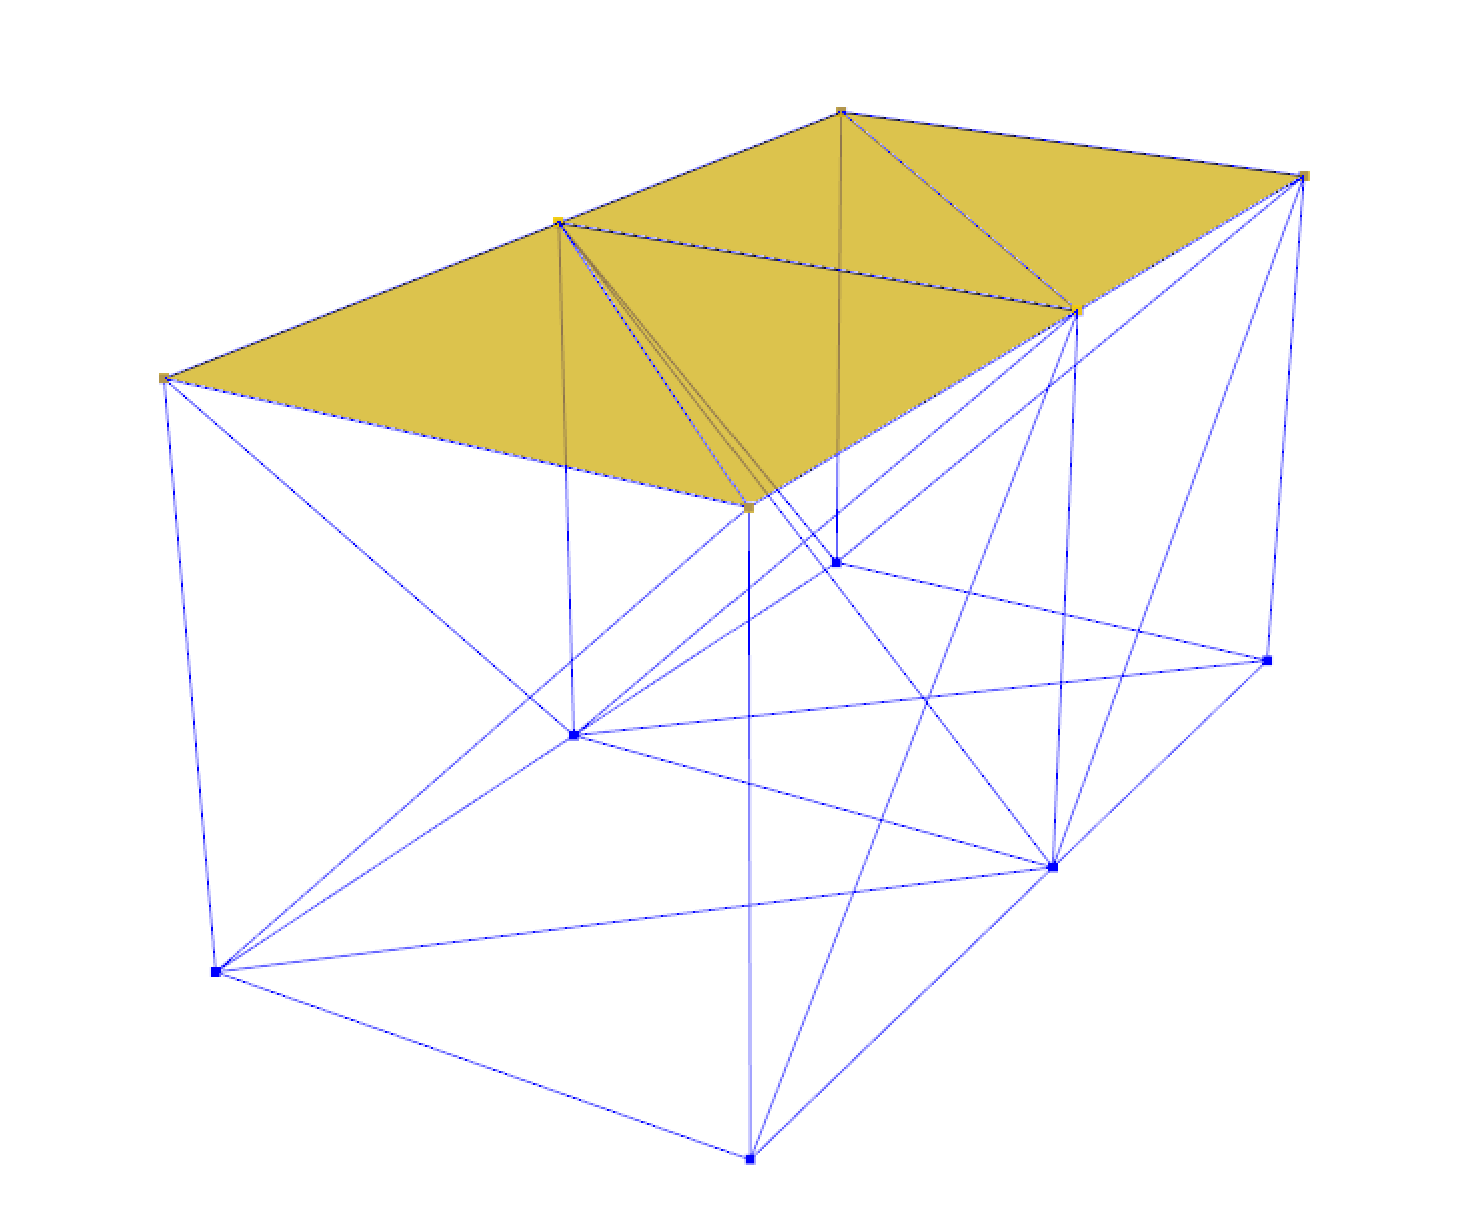
\includegraphics[width=\textwidth]{FOTOS/2.png}
        \caption{Reticulado de 2 módulos.}
    \end{minipage}
    \hfill
    \begin{minipage}[b]{0.5\textwidth}
        \centering
        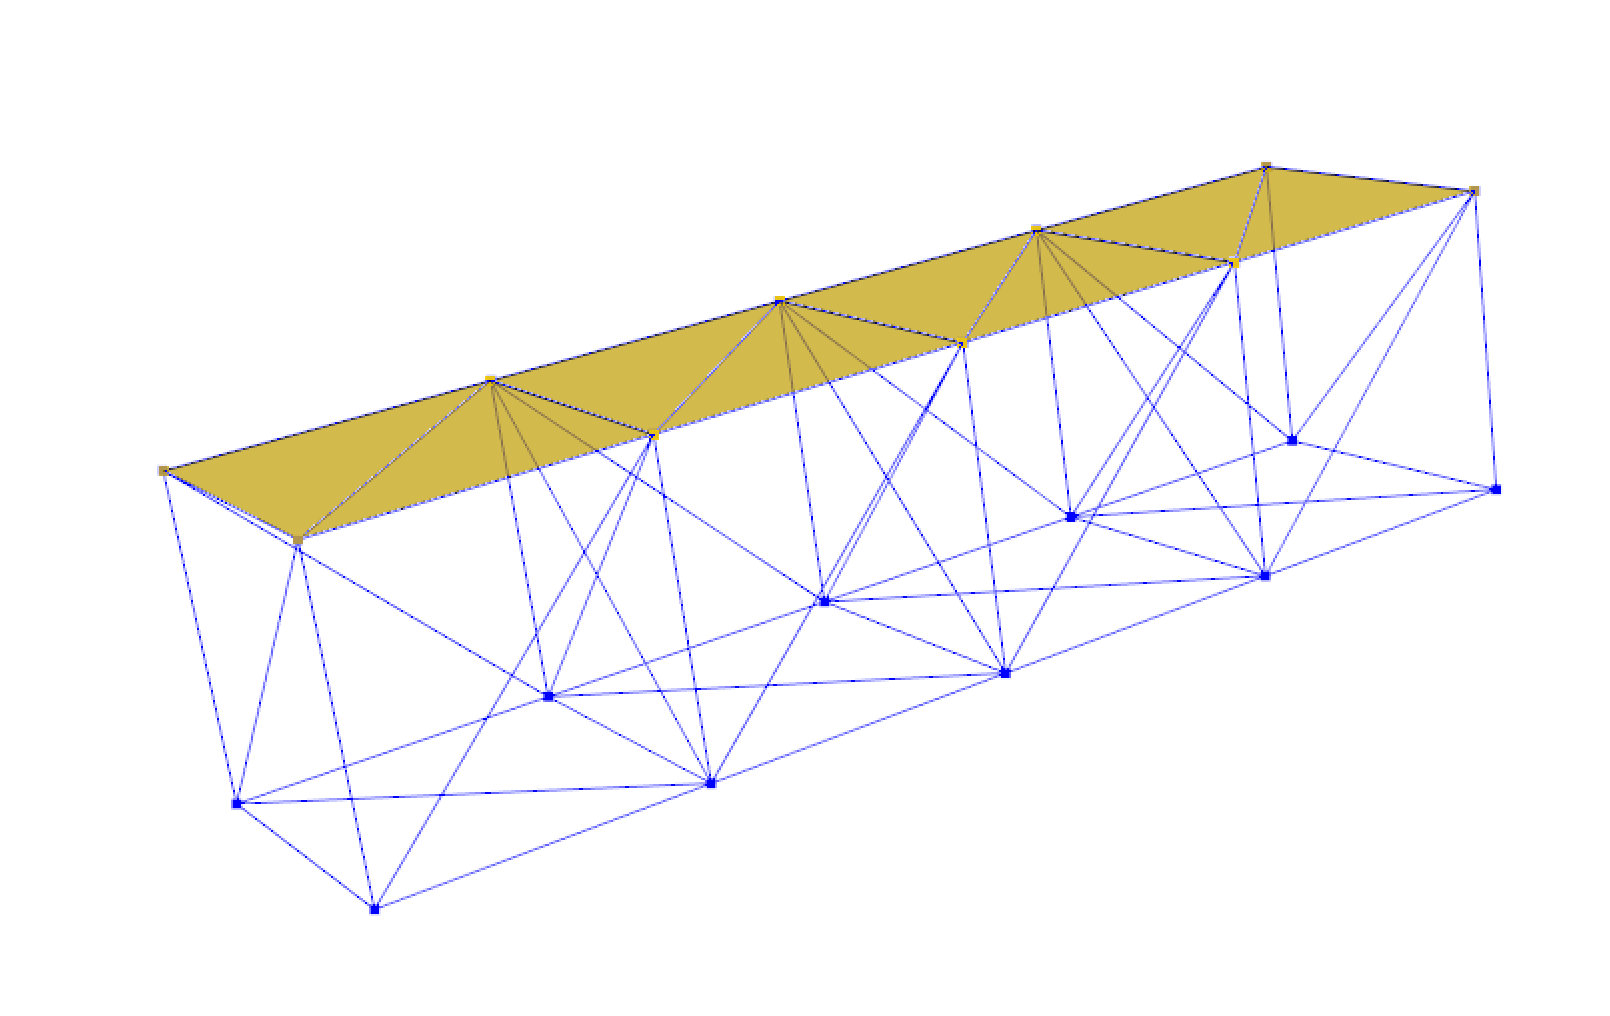
\includegraphics[width=\textwidth]{FOTOS/4.png}
        \caption{Reticulado de 4 módulos.}
    \end{minipage}
\end{figure}

\begin{figure}[H]
    \begin{minipage}[b]{0.5\textwidth}
        \centering
        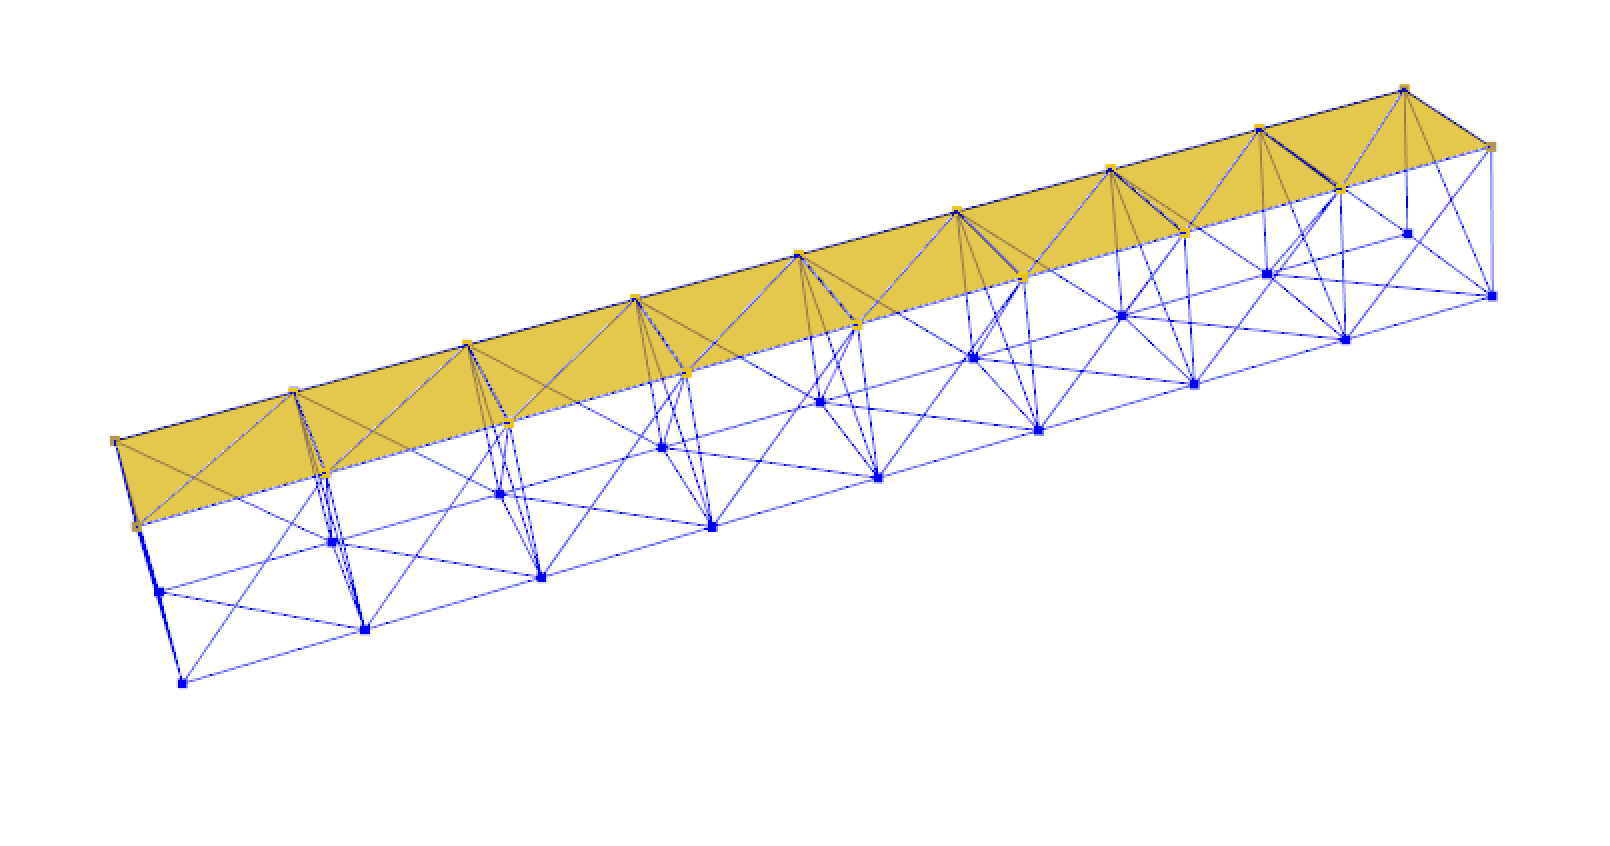
\includegraphics[width=\textwidth]{FOTOS/8.png}
        \caption{Reticulado de 8 módulos.}
    \end{minipage}
    \hfill
    \begin{minipage}[b]{0.5\textwidth}
        \centering
        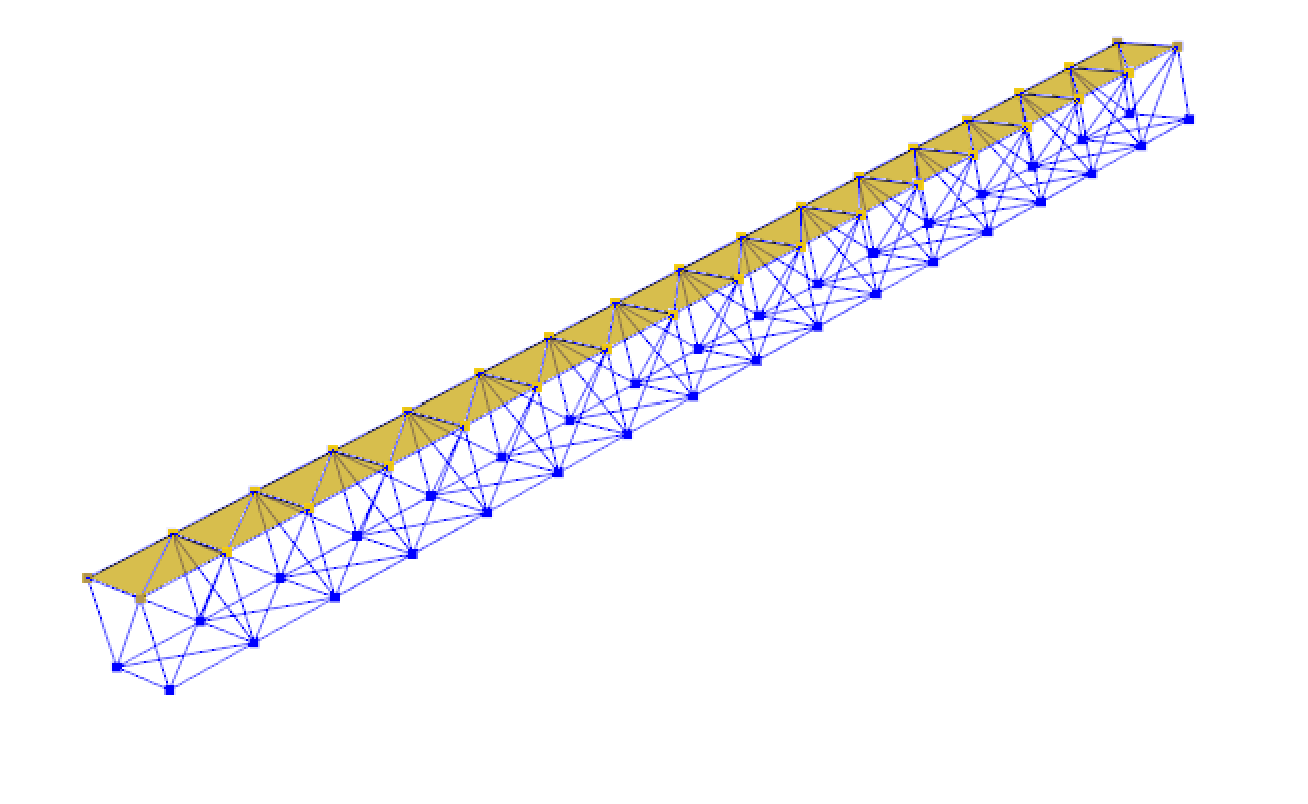
\includegraphics[width=\textwidth]{FOTOS/16.png}
        \caption{Reticulado de 16 módulos.}
    \end{minipage}
\end{figure}

Luego, se procedió a la obtención de las frecuencias y modos de vibración de la estructura, para lo cual se utilizó el comando \texttt{eigen} de OpenSeesPy. Con los datos obtenidos, se procedió a la visualización de los modos de vibración de la estructura, para lo cual se utilizó PyVista. A continuación, se muestran las estructuras con su deformación en el modo 1 de vibración, como ejemplo.

\begin{figure}[H]
    \begin{minipage}[b]{0.5\textwidth}
        \centering
        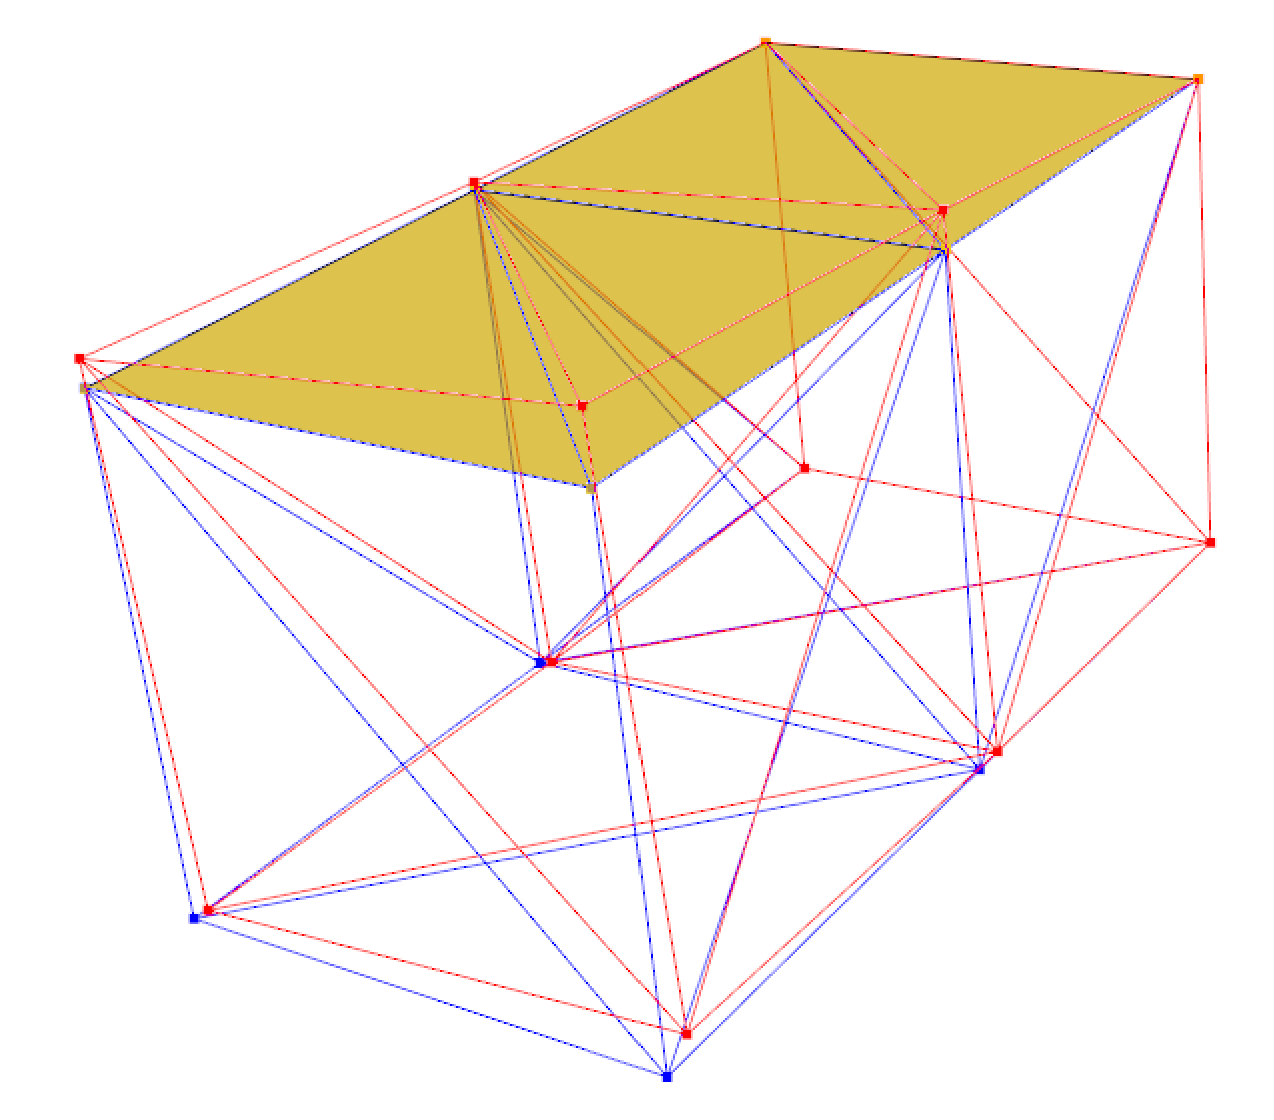
\includegraphics[width=\textwidth]{FOTOS/m1_2.png}
        \caption{Reticulado de 2 y su modo 1.}
    \end{minipage}
    \hfill
    \begin{minipage}[b]{0.5\textwidth}
        \centering
        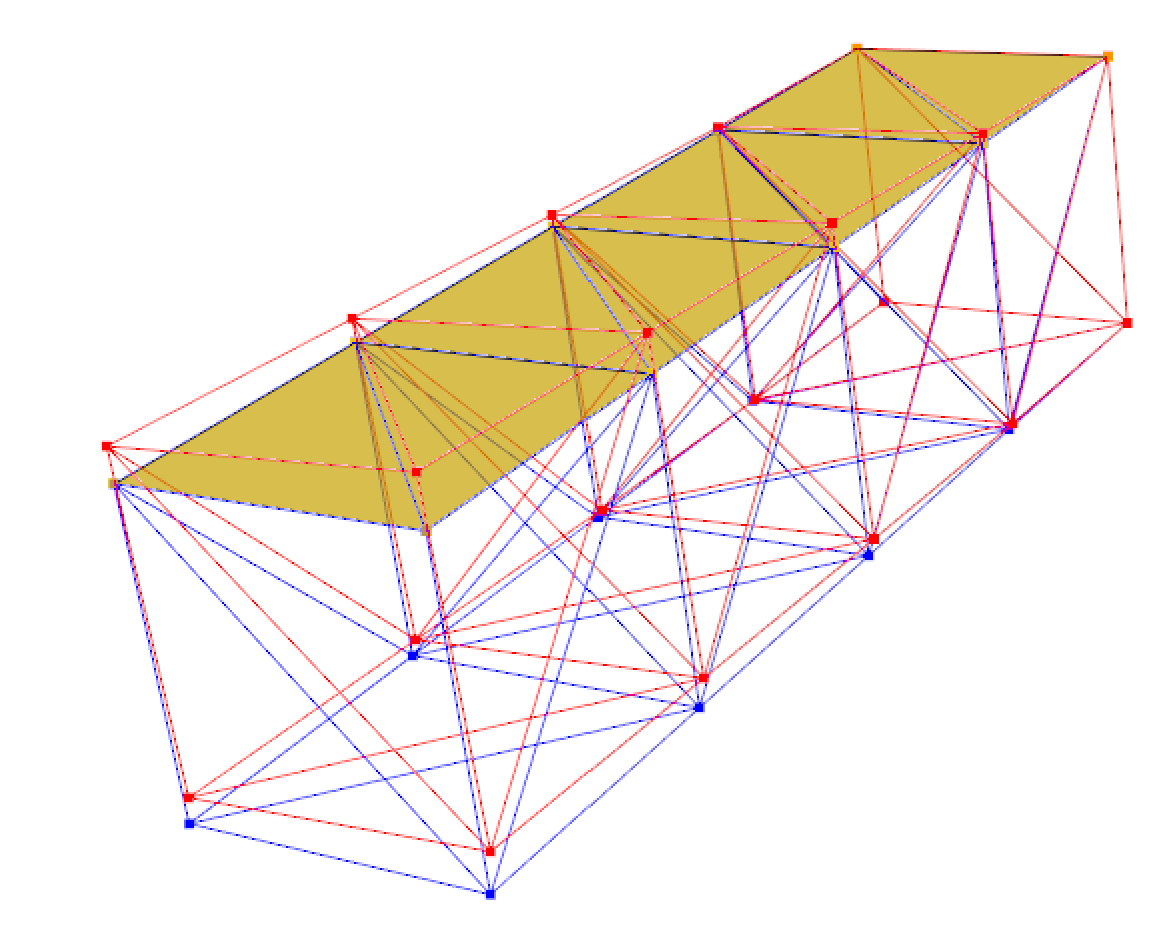
\includegraphics[width=\textwidth]{FOTOS/m1_4.png}
        \caption{Reticulado de 4 y su modo 1.}
    \end{minipage}
\end{figure}

\begin{figure}[H]
    \begin{minipage}[b]{0.5\textwidth}
        \centering
        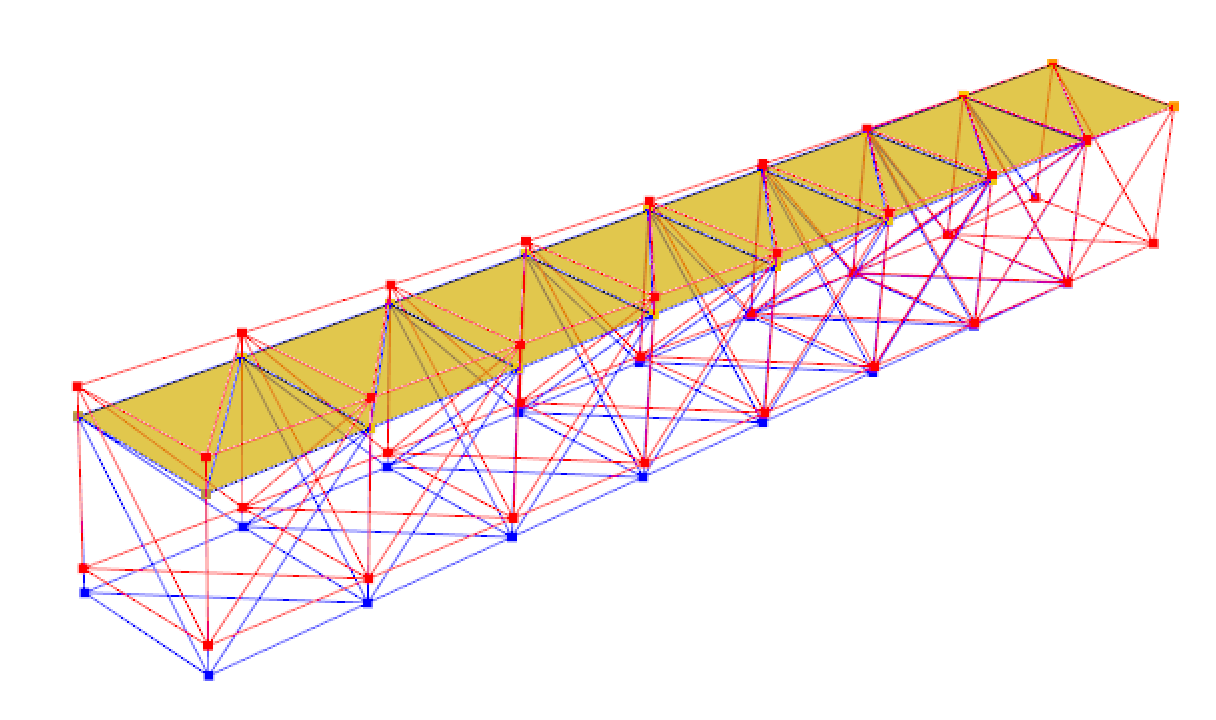
\includegraphics[width=\textwidth]{FOTOS/m1_8.png}
        \caption{Reticulado de 8 y su modo 1.}
    \end{minipage}
    \hfill
    \begin{minipage}[b]{0.5\textwidth}
        \centering
        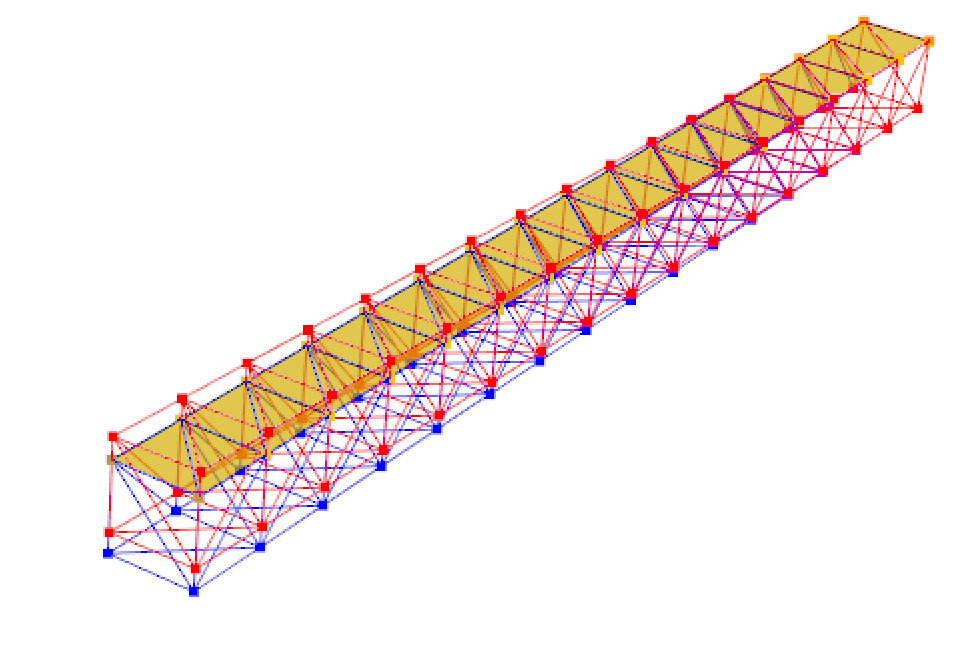
\includegraphics[width=\textwidth]{FOTOS/m1_16.png}
        \caption{Reticulado de 16 y su modo 1.}
    \end{minipage}
\end{figure}

Posteriormente, se procedió a calcular la relación de masa estructural con respecto a los paneles solares, para lo cual se utilizó la siguiente fórmula:

\begin{equation}
    \text{RME} = \frac{\text{Masa de la estructura}}{\text{Masa de los paneles solares}} \cdot 100
\end{equation}

Finalmente, se fueron calibrando los diámetros internos y externos de los tubos de la estructura, para obtener una relación de masa estructural que cumpliera con los siguientes porcentajes: 10\%, 20\%, 30\%

\section{Resultados}


\subsection{Caso de 2 vanos}
En el caso de 2 vanos se obtuvieron los siguientes diámetros de las barras de fibra de carbono, además, se muestran los porcentajes de RME.

\begin{table}[H]
    \centering
    \begin{tabular}{cccc}
    \toprule
     A & Diámetro exterior [mm] & Diámetro interior [mm] & RME [\%] \\
    \midrule
     $A_{10\%}$ &  4 &  2.6 &  10.89 \\
     $A_{20\%}$ &  5 &  2.5 &  22.11 \\
     $A_{30\%}$ &  5.8 &  2.4 &  32.88 \\
    \bottomrule
    \end{tabular}
\end{table}

Donde se obtuvieron las siguientes frecuencias de vibración para cada porcentaje de RME.

\begin{table}[H]
    \centering
    \begin{tabular}{cccc}
    \toprule
     Frecuencia (Hz) & $A_{10\%}$ & $A_{20\%}$ & $A_{30\%}$ \\
    \midrule
     1 &  0.245 &  0.349 &  0.425 \\
     2 &  0.283 &  0.400 &  0.484 \\
     3 &  0.314 &  0.445 &  0.540 \\
     4 &  0.666 &  0.947 &  1.154 \\
     5 &  0.673 &  0.958 &  1.166 \\
     6 &  0.744 &  1.054 &  1.280 \\
     7 &  1.014 &  1.442 &  1.757 \\
     8 &  1.046 &  1.488 &  1.812 \\
     9 &  1.206 &  1.717 &  2.092 \\
     10 &  1.454 &  2.070 &  2.522 \\
    \bottomrule
    \end{tabular}
\end{table}

En este caso todas las combinaciones logran la frecuencia fundamental esperada, ya que en todos los casos es mayor a 0.1 Hz. Además, se puede observar que a medida que aumenta el porcentaje de RME, las frecuencias también aumentan.

A continuación se muestra un gráfico de la frecuencia para cada modo de vibración y cada RME. 

\begin{figure}[H]
    \centering
    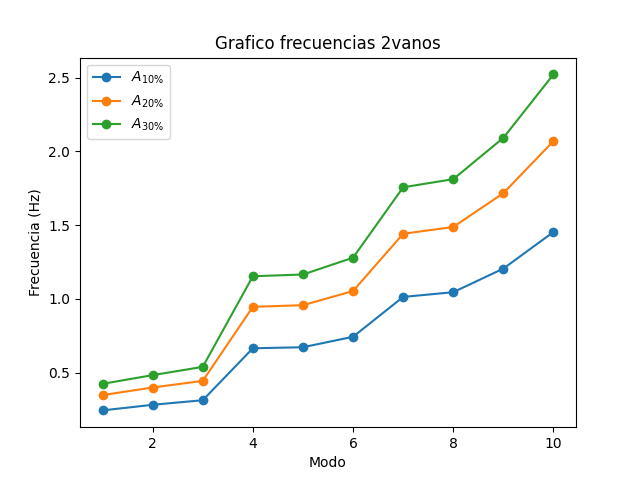
\includegraphics[width=0.8\textwidth]{../grafico_frecuencias_2vanos.png}
    \caption{Frecuencia de vibración para cada modo de vibración y cada RME.}
\end{figure}

\subsection{Caso de 4 vanos}
En el caso de 4 vanos se obtuvieron los siguientes diámetros de las barras de fibra de carbono, además, se muestran los porcentajes de RME.

\begin{table}[H]
    \centering
    \begin{tabular}{cccc}
    \toprule
     A & Diámetro exterior [mm] & Diámetro interior [mm] & RME [\%] \\
    \midrule
     $A_{10\%}$ &  4 &  2.6 &  10.41 \\
     $A_{20\%}$ &  5 &  2.5 &  21.13 \\
     $A_{30\%}$ &  5.8 &  2.4 &  31.41 \\
    \bottomrule
    \end{tabular}
\end{table}

Donde se obtuvieron las siguientes frecuencias de vibración para cada porcentaje de RME.

\begin{table}[H]
    \centering
    \begin{tabular}{cccc}
    \toprule
     Frecuencia (Hz) & $A_{10\%}$ & $A_{20\%}$ & $A_{30\%}$ \\
    \midrule
     1 &       0.103 &       0.146 &       0.175 \\
     2 &       0.141 &       0.195 &       0.228 \\
     3 &       0.162 &       0.228 &       0.272 \\
     4 &       0.342 &       0.486 &       0.582 \\
     5 &       0.393 &       0.553 &       0.656 \\
     6 &       0.449 &       0.633 &       0.754 \\
     7 &       0.597 &       0.849 &       1.015 \\
     8 &       0.624 &       0.887 &       1.060 \\
     9 &       0.688 &       0.974 &       1.162 \\
     10 &       0.735 &       1.039 &       1.236 \\
    \bottomrule
    \end{tabular}
\end{table}

En este caso se puede observar que todas las combinaciones logran la frecuencia esperada, ya que todas son mayores a 0.1 Hz.

A continuación, se muestra el gráfico de la frecuencia para cada modo de vibración y cada RME. 

\begin{figure}[H]
    \centering
    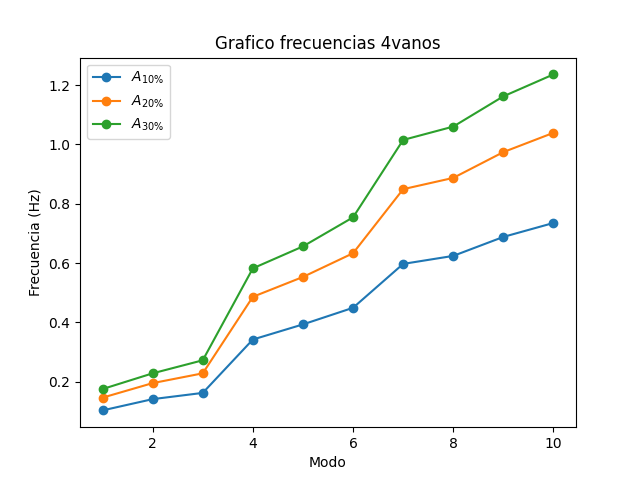
\includegraphics[width=0.8\textwidth]{../grafico_frecuencias_4vanos.png}
    \caption{Frecuencia de vibración para cada modo de vibración y cada RME.}
\end{figure}

Junto a esto, se obtuvieron los gráficos de los 10 primeros modos de vibración de la estructura (N=4).

\begin{figure}[H]
    \begin{minipage}[b]{0.5\textwidth}
        \centering
        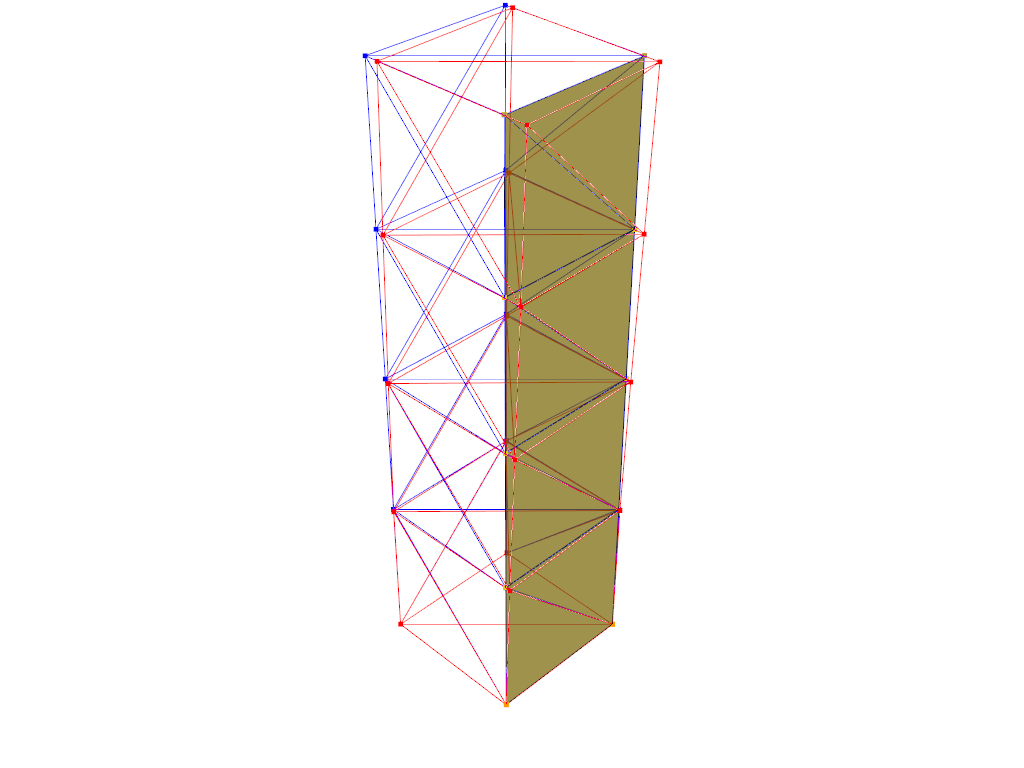
\includegraphics[width=\textwidth]{FOTOS/mod1_4.png}
        \caption{Primer modo de vibración N=4.}
    \end{minipage}
    \hfill
    \begin{minipage}[b]{0.5\textwidth}
        \centering
        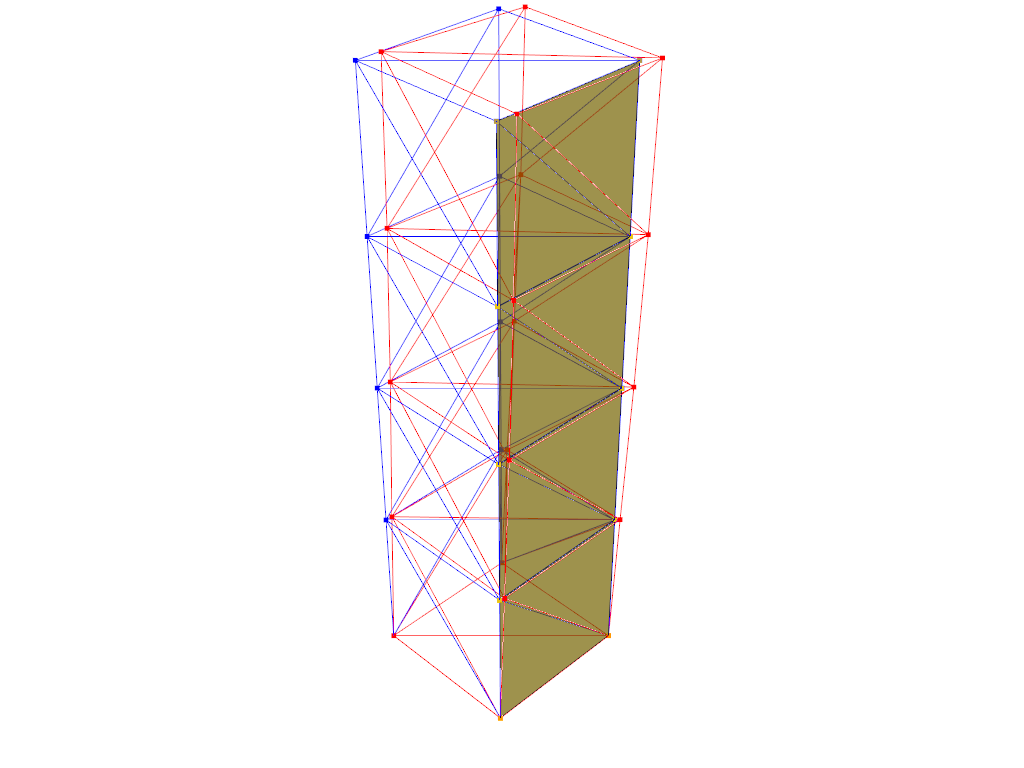
\includegraphics[width=\textwidth]{FOTOS/mod2_4.png}
        \caption{Segundo modo de vibración N=4.}
    \end{minipage}
\end{figure}

\begin{figure}[H]
    \begin{minipage}[b]{0.5\textwidth}
        \centering
        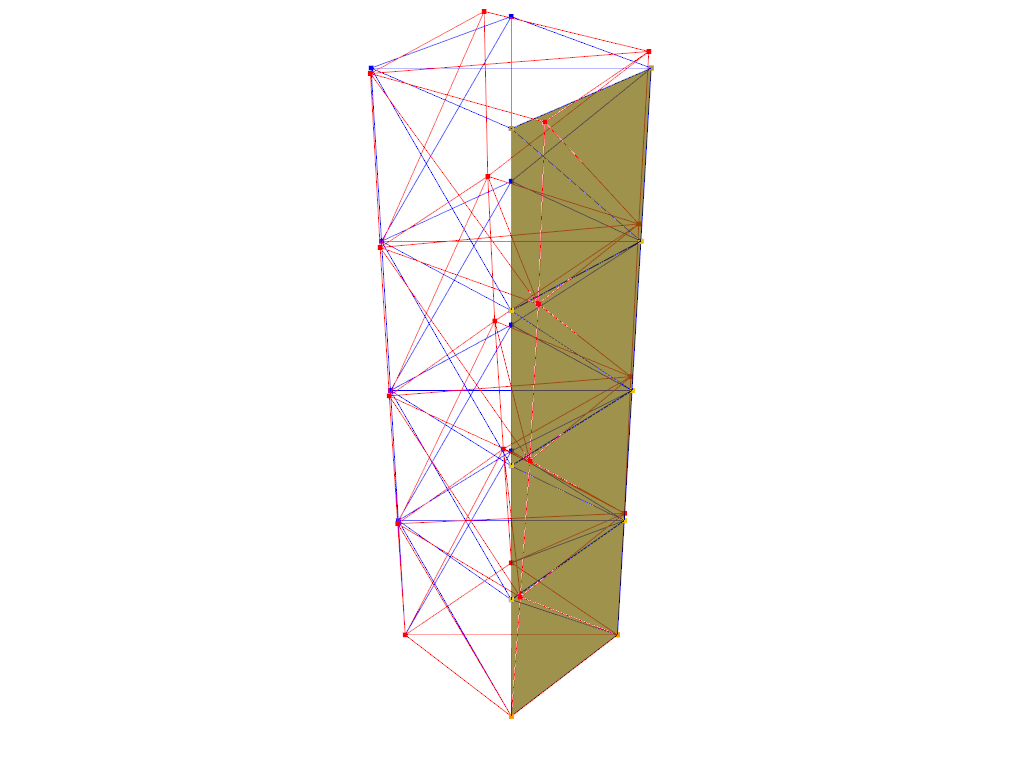
\includegraphics[width=\textwidth]{FOTOS/mod3_4.png}
        \caption{Tercer modo de vibración N=4.}
    \end{minipage}
    \hfill
    \begin{minipage}[b]{0.5\textwidth}
        \centering
        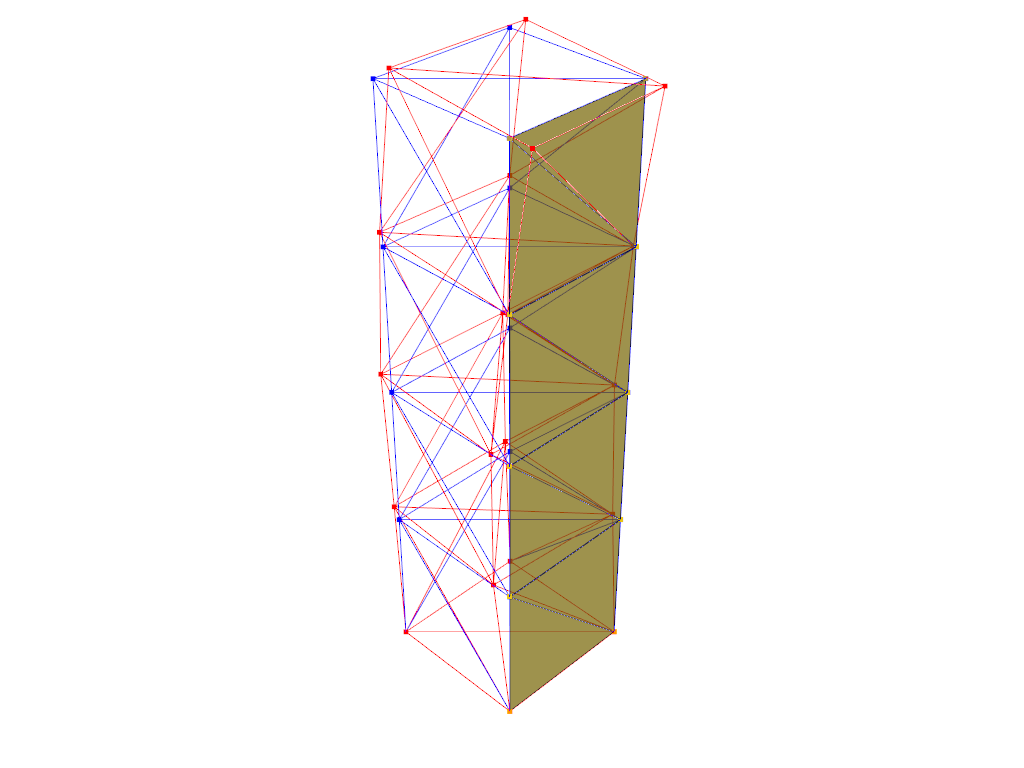
\includegraphics[width=\textwidth]{FOTOS/mod4_4.png}
        \caption{Cuarto modo de vibración N=4.}
    \end{minipage}
\end{figure}

\begin{figure}[H]
    \begin{minipage}[b]{0.5\textwidth}
        \centering
        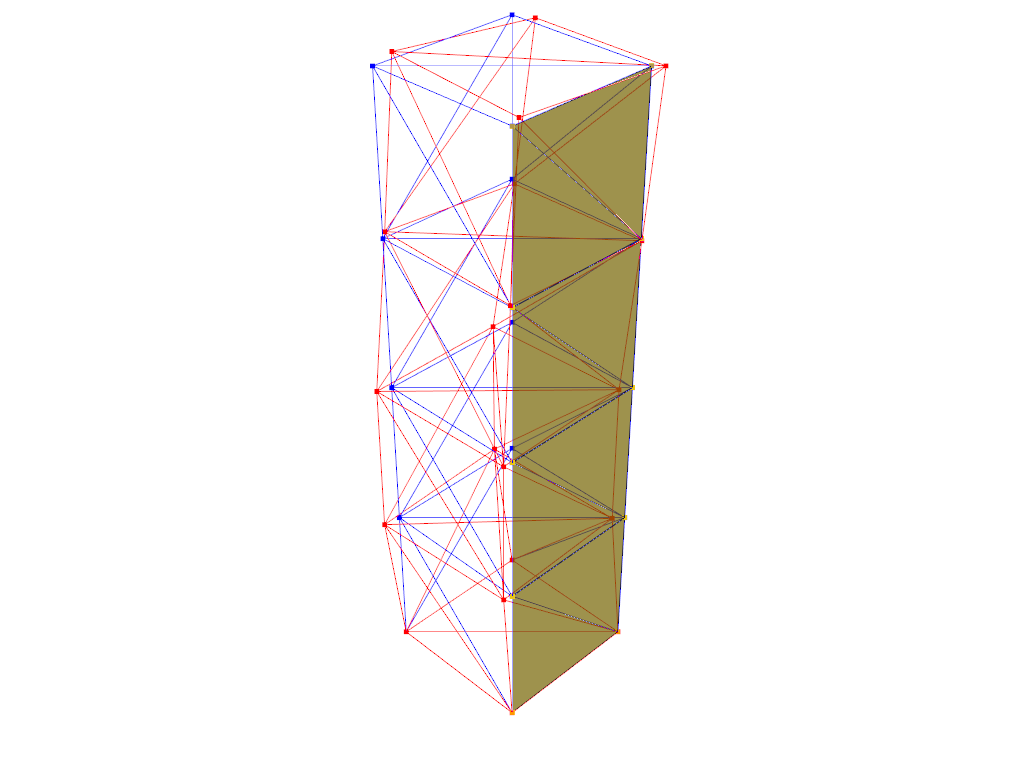
\includegraphics[width=\textwidth]{FOTOS/mod5_4.png}
        \caption{Quinto modo de vibración N=4.}
    \end{minipage}
    \hfill
    \begin{minipage}[b]{0.5\textwidth}
        \centering
        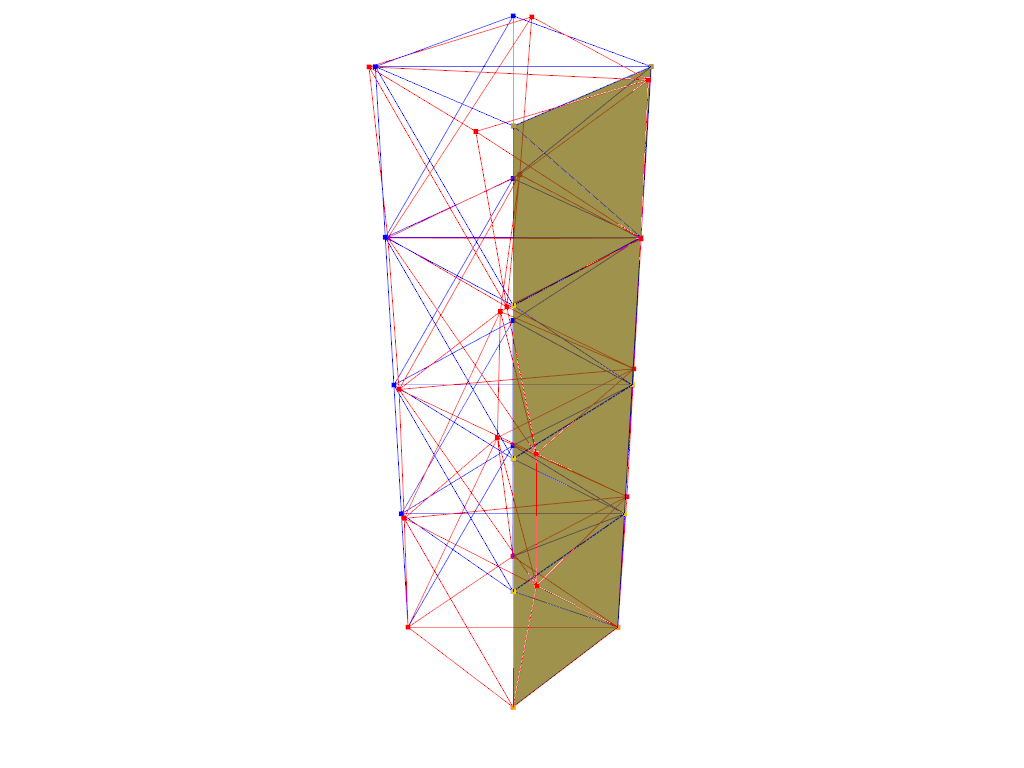
\includegraphics[width=\textwidth]{FOTOS/mod6_4.png}
        \caption{Sexto modo de vibración N=4.}
    \end{minipage}
\end{figure}

\begin{figure}[H]
    \begin{minipage}[b]{0.5\textwidth}
        \centering
        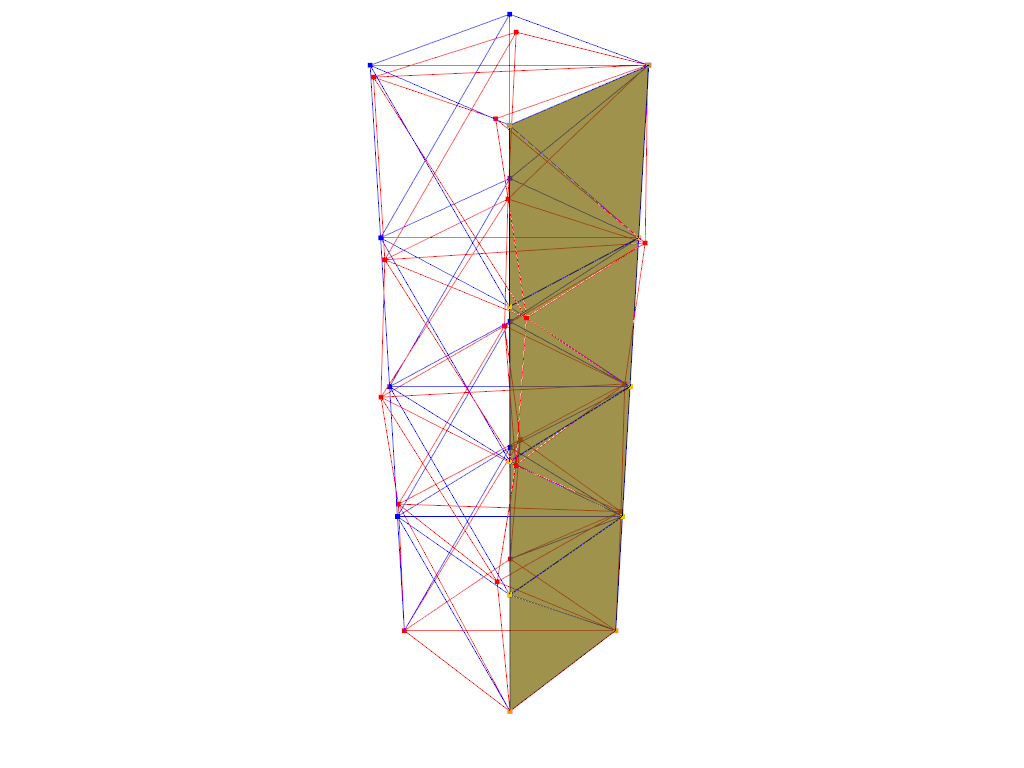
\includegraphics[width=\textwidth]{FOTOS/mod7_4.png}
        \caption{Séptimo modo de vibración N=4.}
    \end{minipage}
    \hfill
    \begin{minipage}[b]{0.5\textwidth}
        \centering
        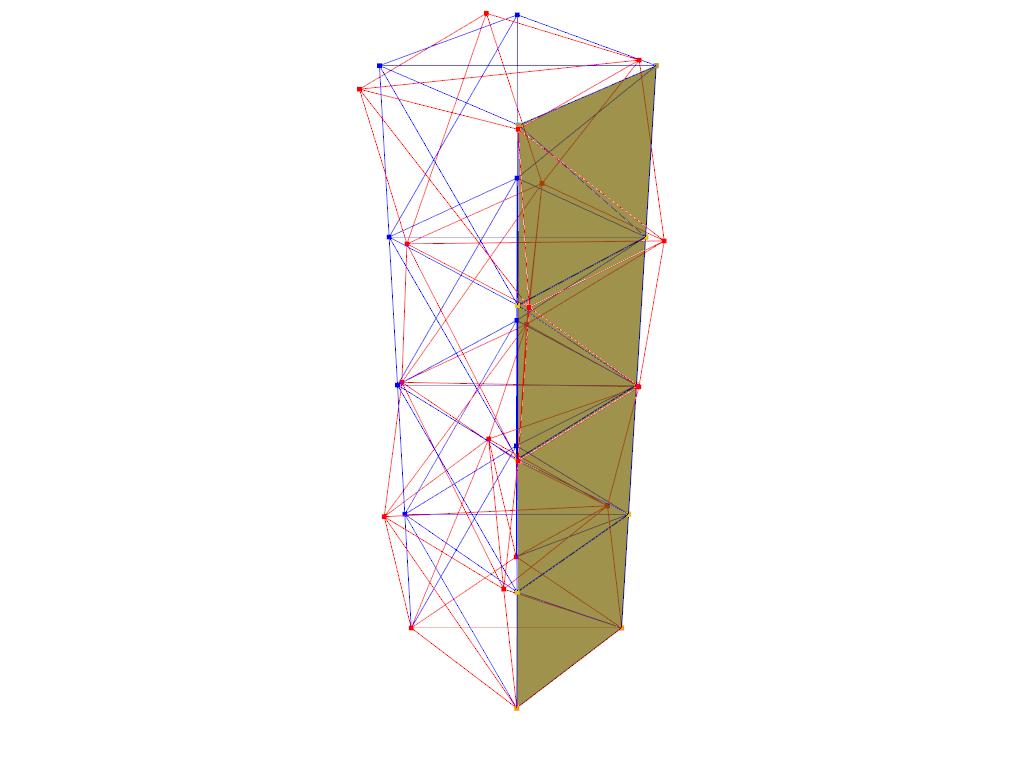
\includegraphics[width=\textwidth]{FOTOS/mod8_4.png}
        \caption{Octavo modo de vibración N=4.}
    \end{minipage}
\end{figure}

\begin{figure}[H]
    \begin{minipage}[b]{0.5\textwidth}
        \centering
        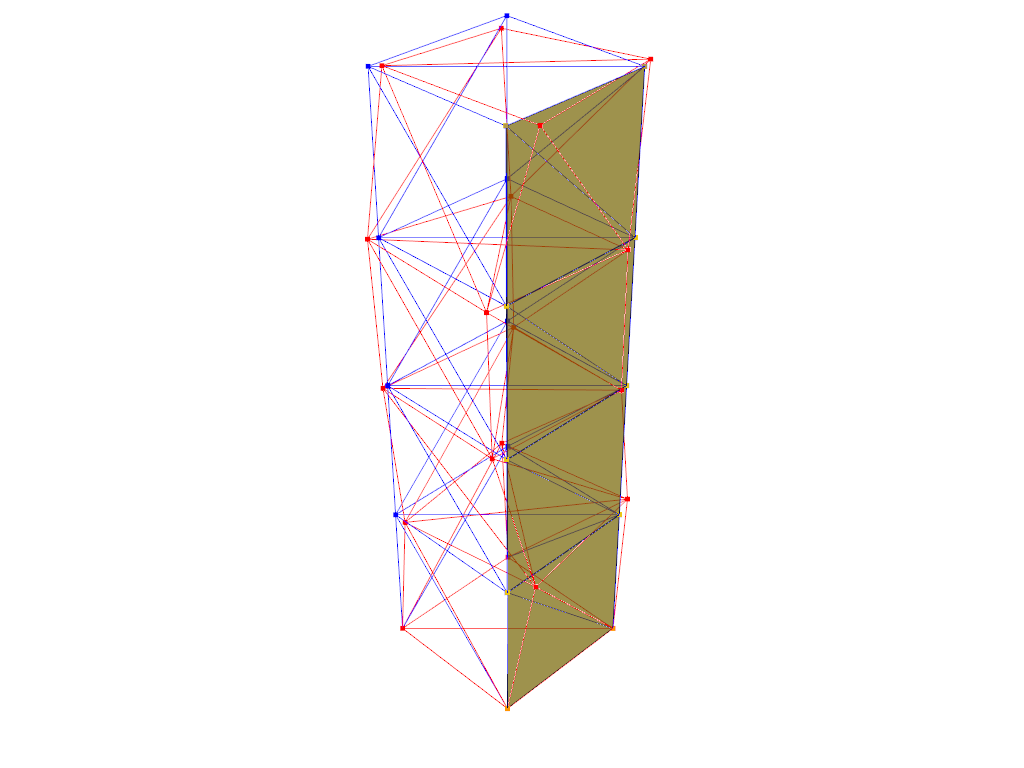
\includegraphics[width=\textwidth]{FOTOS/mod9_4.png}
        \caption{Noveno modo de vibración N=4.}
    \end{minipage}
    \hfill
    \begin{minipage}[b]{0.5\textwidth}
        \centering
        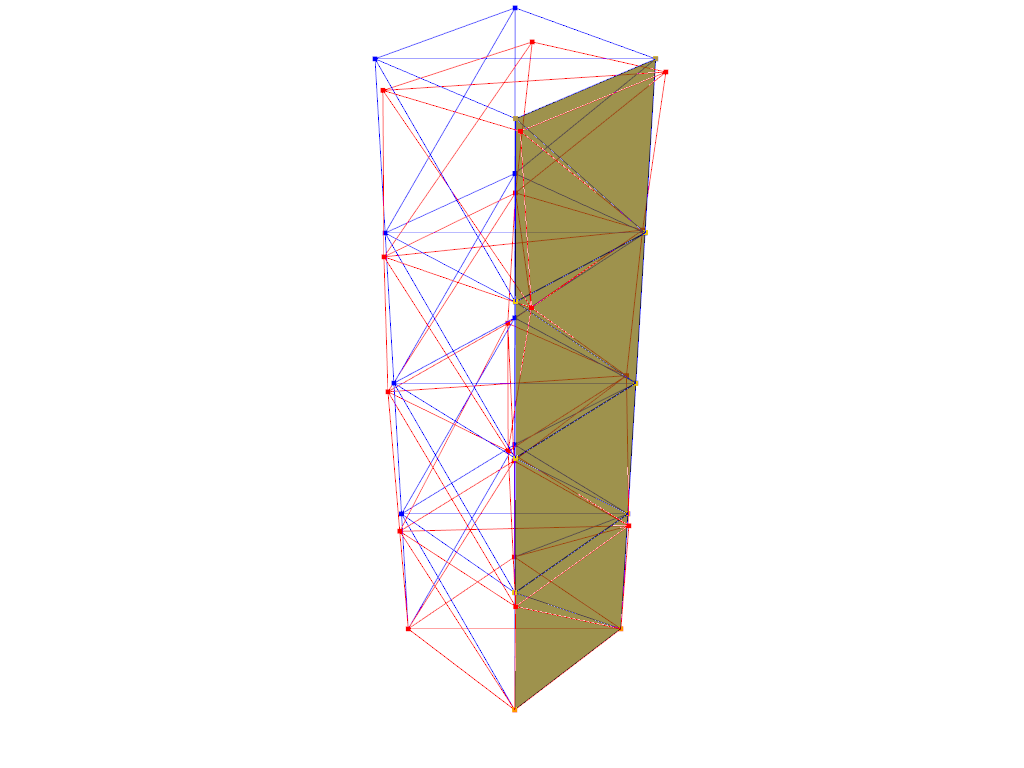
\includegraphics[width=\textwidth]{FOTOS/mod10_4.png}
        \caption{Décimo modo de vibración N=4.}
    \end{minipage}
\end{figure}

\subsection{Caso de 8 vanos}
En el caso de 8 vanos se obtuvieron los siguientes diámetros de las barras de fibra de carbono, además, se muestran los porcentajes de RME.

\begin{table}[H]
    \centering
    \begin{tabular}{cccc}
    \toprule
     A & Diámetro exterior [mm] & Diámetro interior [mm] & RME [\%] \\
    \midrule
     $A_{10\%}$ &  4 &  2.6 &  10.17 \\
     $A_{20\%}$ &  5 &  2.5 &  20.63 \\
     $A_{30\%}$ &  5.8 &  2.4 &  30.68 \\
    \bottomrule
    \end{tabular}
\end{table}

Donde se obtuvieron las siguientes frecuencias de vibración para cada porcentaje de RME.

\begin{table}[H]
    \centering
    \begin{tabular}{cccc}
    \toprule
     Frecuencia (Hz) & $A_{10\%}$ & $A_{20\%}$ & $A_{30\%}$ \\
    \midrule
     1 &       0.035 &       0.049 &       0.059 \\
     2 &       0.064 &       0.083 &       0.095 \\
     3 &       0.081 &       0.115 &       0.139 \\
     4 &       0.147 &       0.208 &       0.253 \\
     5 &       0.195 &       0.266 &       0.314 \\
     6 &       0.234 &       0.330 &       0.399 \\
     7 &       0.307 &       0.435 &       0.528 \\
     8 &       0.336 &       0.474 &       0.574 \\
     9 &       0.388 &       0.548 &       0.663 \\
     10 &       0.444 &       0.629 &       0.760 \\
    \bottomrule
    \end{tabular}
\end{table}

En este caso se puede observar que ninguna de las combinaciones logra la frecuencia fundamental esperada, ya que en todos los casos es menor a 0.1 Hz.

A continuación se muestra un gráfico de la frecuencia para cada modo de vibración y cada RME. 

\begin{figure}[H]
    \centering
    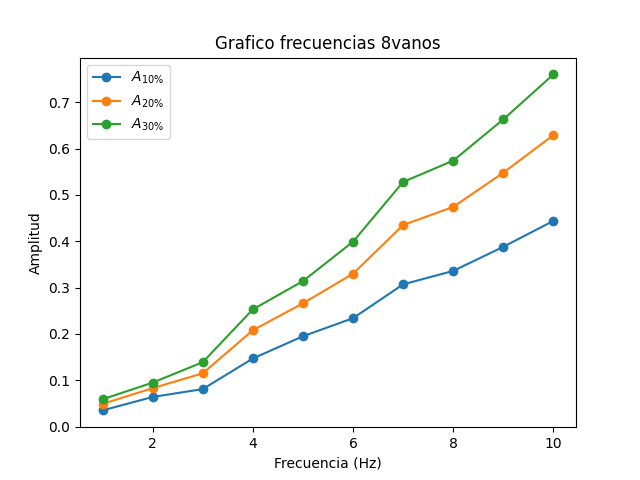
\includegraphics[width=0.8\textwidth]{../grafico_frecuencias_8vanos.png}
    \caption{Frecuencia de vibración para cada modo de vibración y cada RME.}
\end{figure}

\newpage

\subsection{Caso de 16 vanos}
En el caso de 16 vanos se obtuvieron los siguientes diámetros de las barras de fibra de carbono, además, se muestran los porcentajes de RME.

\begin{table}[H]
    \centering
    \begin{tabular}{cccc}
    \toprule
     A & Diámetro exterior [mm] & Diámetro interior [mm] & RME [\%] \\
    \midrule
     $A_{10\%}$ &  4 &  2.6 &  10.05 \\
     $A_{20\%}$ &  5 &  2.5 &  20.39 \\
     $A_{30\%}$ &  5.8 &  2.4 &  30.32 \\
    \bottomrule
    \end{tabular}
\end{table}

Donde se obtuvieron las siguientes frecuencias de vibración para cada porcentaje de RME.

\begin{table}[H]
    \centering
    \begin{tabular}{cccc}
    \toprule
     Frecuencia (Hz) & $A_{10\%}$ & $A_{20\%}$ & $A_{30\%}$ \\
    \midrule
     1 &       0.010 &       0.014 &       0.017 \\
     2 &       0.025 &       0.029 &       0.031 \\
     3 &       0.040 &       0.057 &       0.069 \\
     4 &       0.052 &       0.074 &       0.090 \\
     5 &       0.086 &       0.112 &       0.130 \\
     6 &       0.113 &       0.160 &       0.194 \\
     7 &       0.130 &       0.184 &       0.223 \\
     8 &       0.161 &       0.222 &       0.264 \\
     9 &       0.192 &       0.270 &       0.326 \\
     10 &       0.212 &       0.299 &       0.363 \\
    \bottomrule
    \end{tabular}
\end{table}

En este caso se puede observar que ninguna de las combinaciones logra la frecuencia fundamental esperada, ya que en todos los casos es menor a 0.1 Hz.

A continuación se muestra un gráfico de la frecuencia para cada modo de vibración y cada RME. 

\begin{figure}[H]
    \centering
    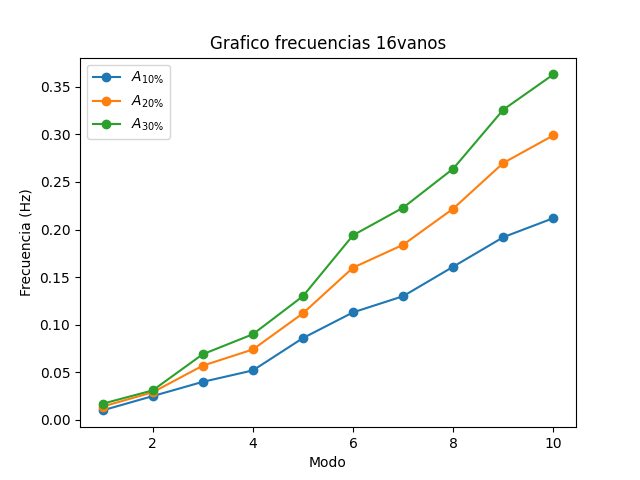
\includegraphics[width=0.8\textwidth]{../grafico_frecuencias_16vanos.png}
    \caption{Frecuencia de vibración para cada modo de vibración y cada RME.}
\end{figure}

Junto a esto, se obtuvieron los gráficos de los 10 primeros modos de vibración de la estructura (N=16).

\begin{figure}[H]
    \begin{minipage}[b]{0.5\textwidth}
        \centering
        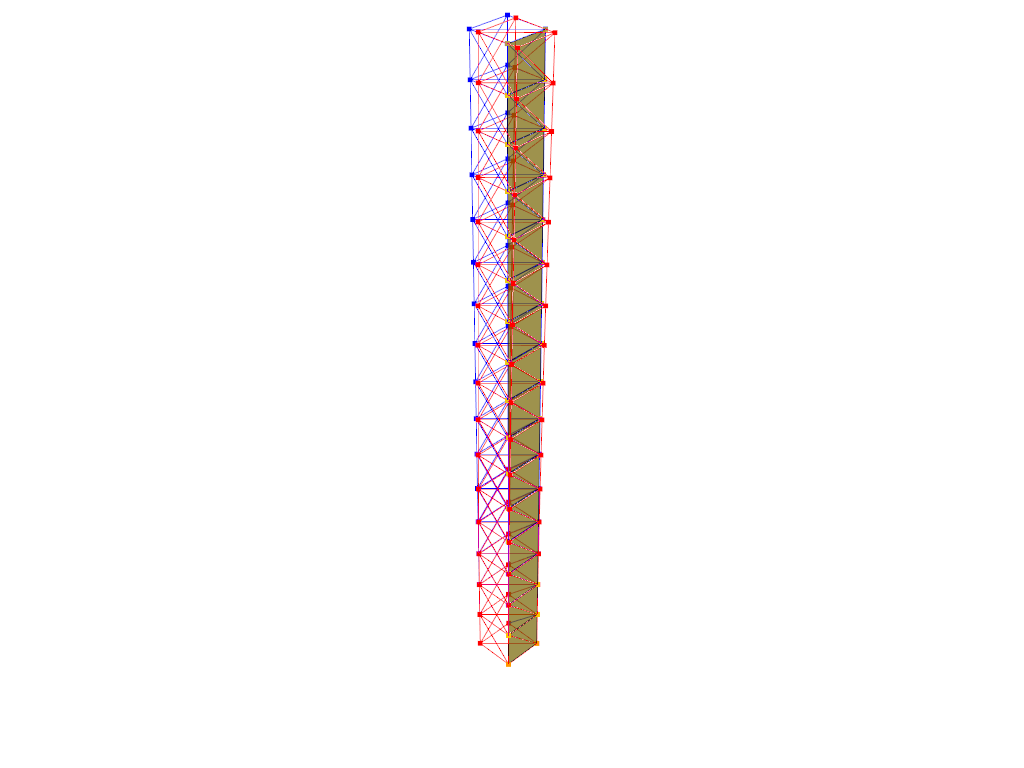
\includegraphics[width=\textwidth]{FOTOS/mod1_16.png}
        \caption{Primer modo de vibración N=16.}
    \end{minipage}
    \hfill
    \begin{minipage}[b]{0.5\textwidth}
        \centering
        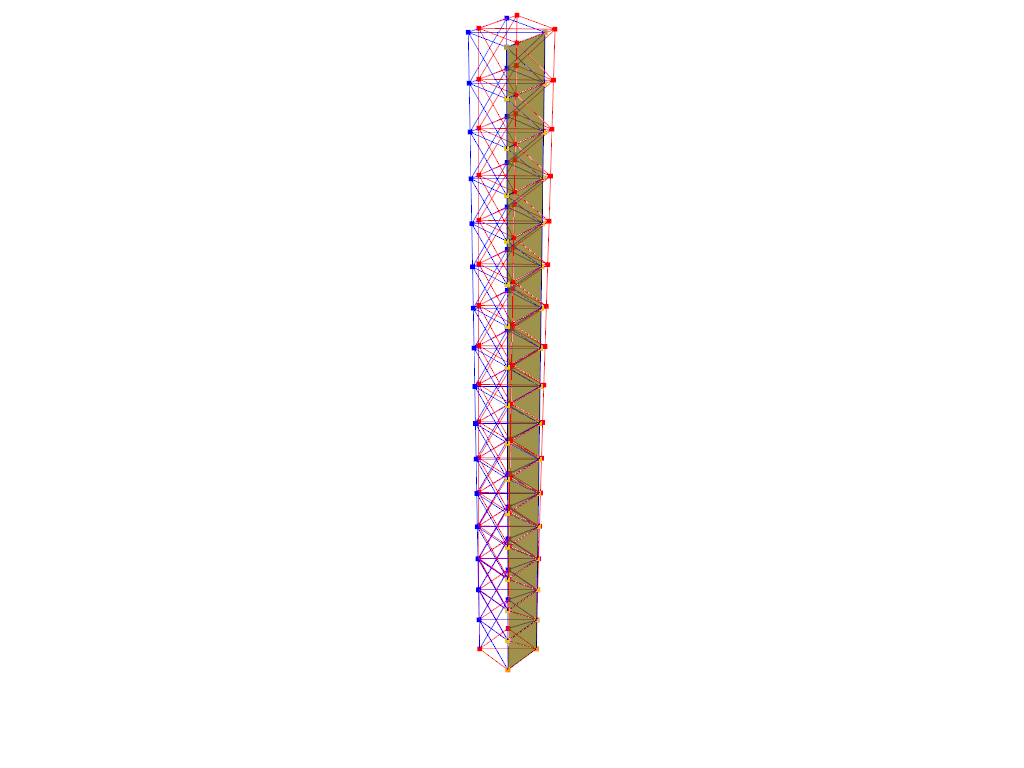
\includegraphics[width=\textwidth]{FOTOS/mod2_16.png}
        \caption{Segundo modo de vibración N=16.}
    \end{minipage}
\end{figure}

\begin{figure}[H]
    \begin{minipage}[b]{0.5\textwidth}
        \centering
        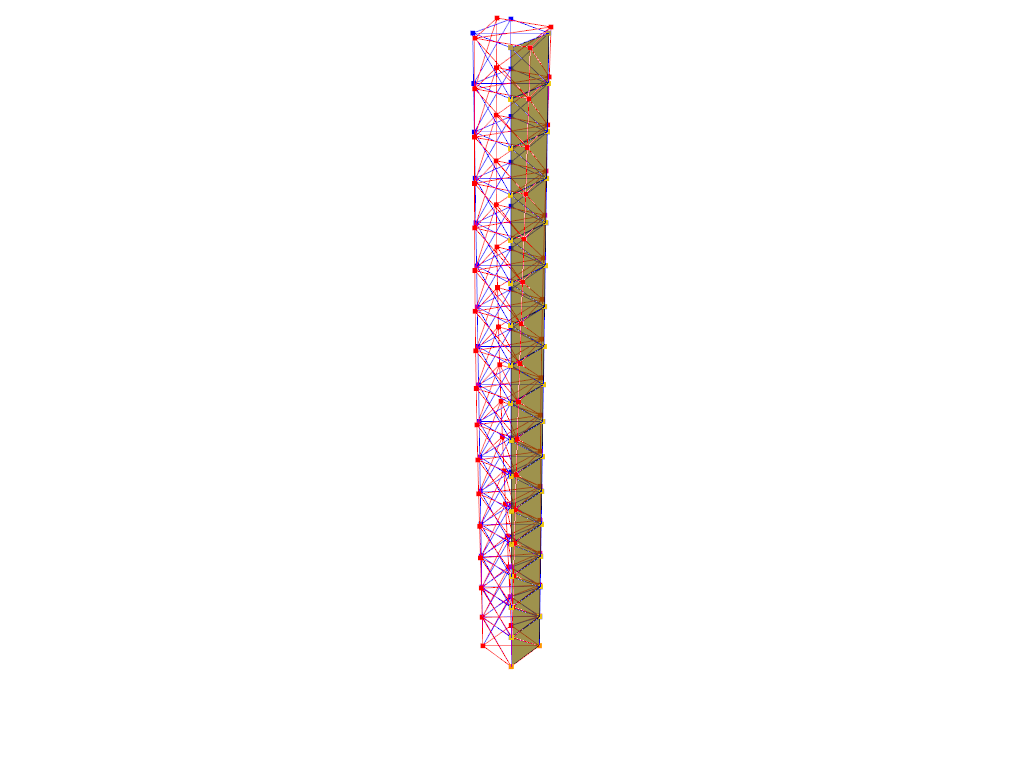
\includegraphics[width=\textwidth]{FOTOS/mod3_16.png}
        \caption{Tercer modo de vibración N=16.}
    \end{minipage}
    \hfill
    \begin{minipage}[b]{0.5\textwidth}
        \centering
        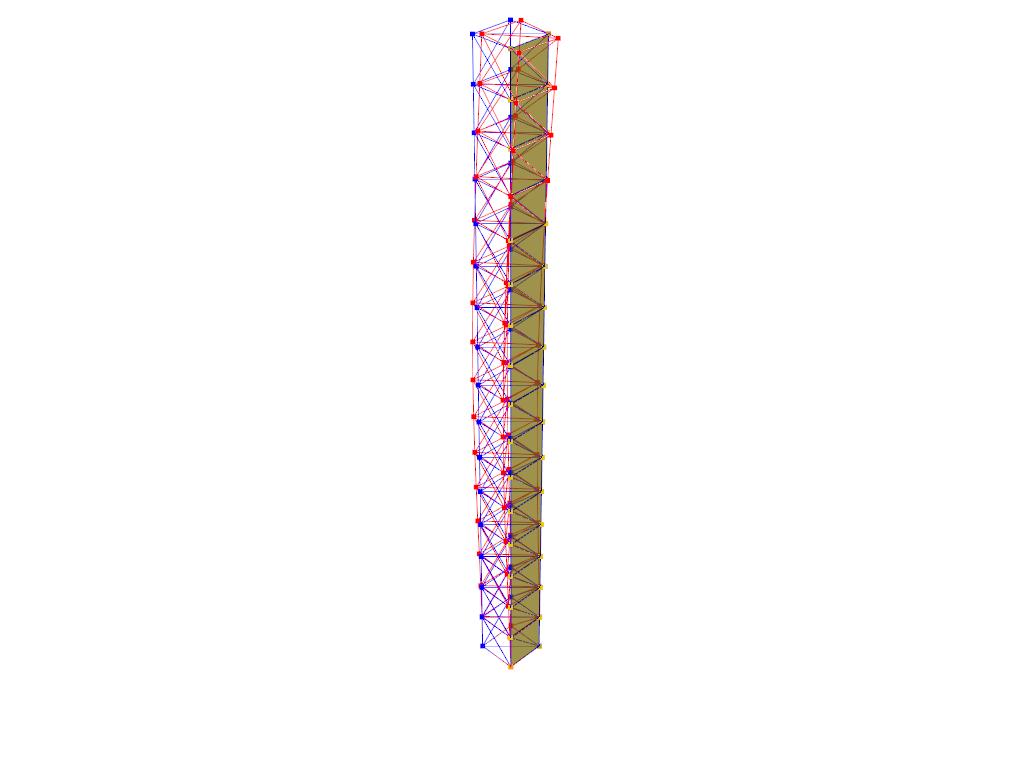
\includegraphics[width=\textwidth]{FOTOS/mod4_16.png}
        \caption{Cuarto modo de vibración N=16.}
    \end{minipage}
\end{figure}

\begin{figure}[H]
    \begin{minipage}[b]{0.5\textwidth}
        \centering
        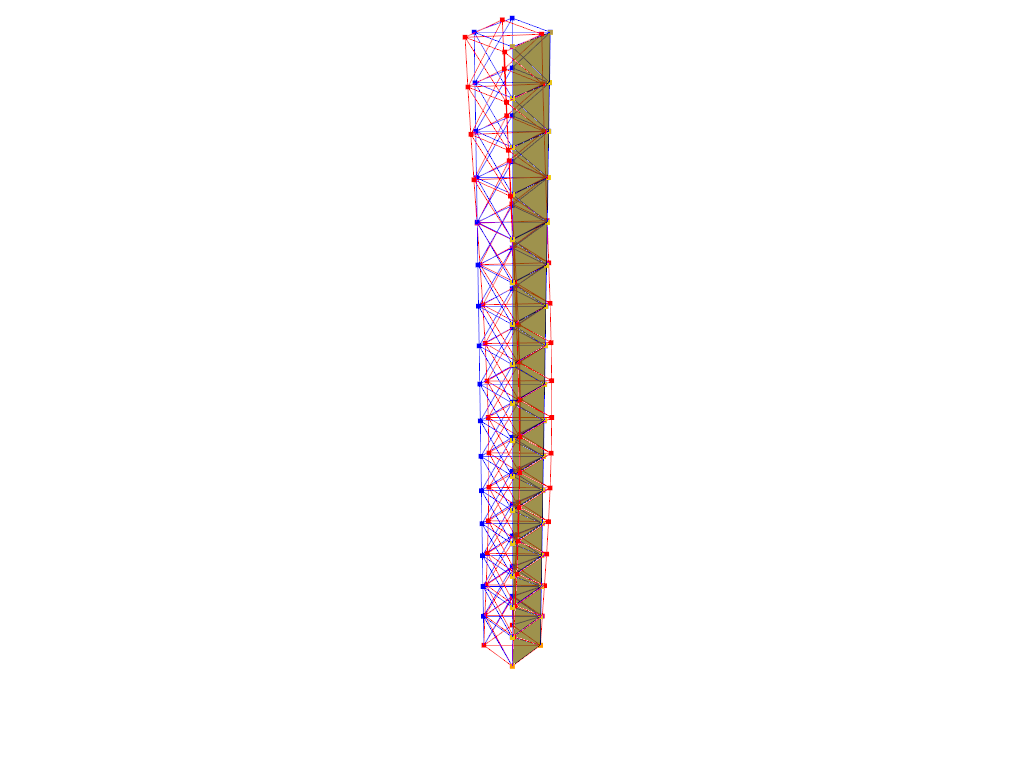
\includegraphics[width=\textwidth]{FOTOS/mod5_16.png}
        \caption{Quinto modo de vibración N=16.}
    \end{minipage}
    \hfill
    \begin{minipage}[b]{0.5\textwidth}
        \centering
        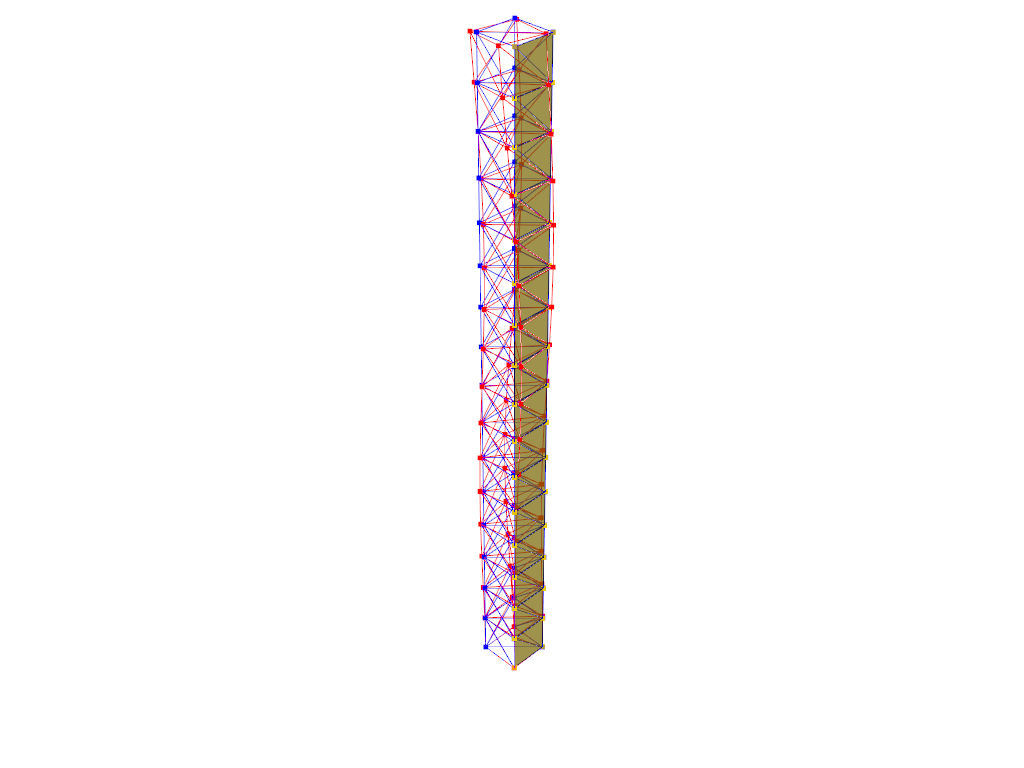
\includegraphics[width=\textwidth]{FOTOS/mod6_16.png}
        \caption{Sexto modo de vibración N=16.}
    \end{minipage}
\end{figure}

\begin{figure}[H]
    \begin{minipage}[b]{0.5\textwidth}
        \centering
        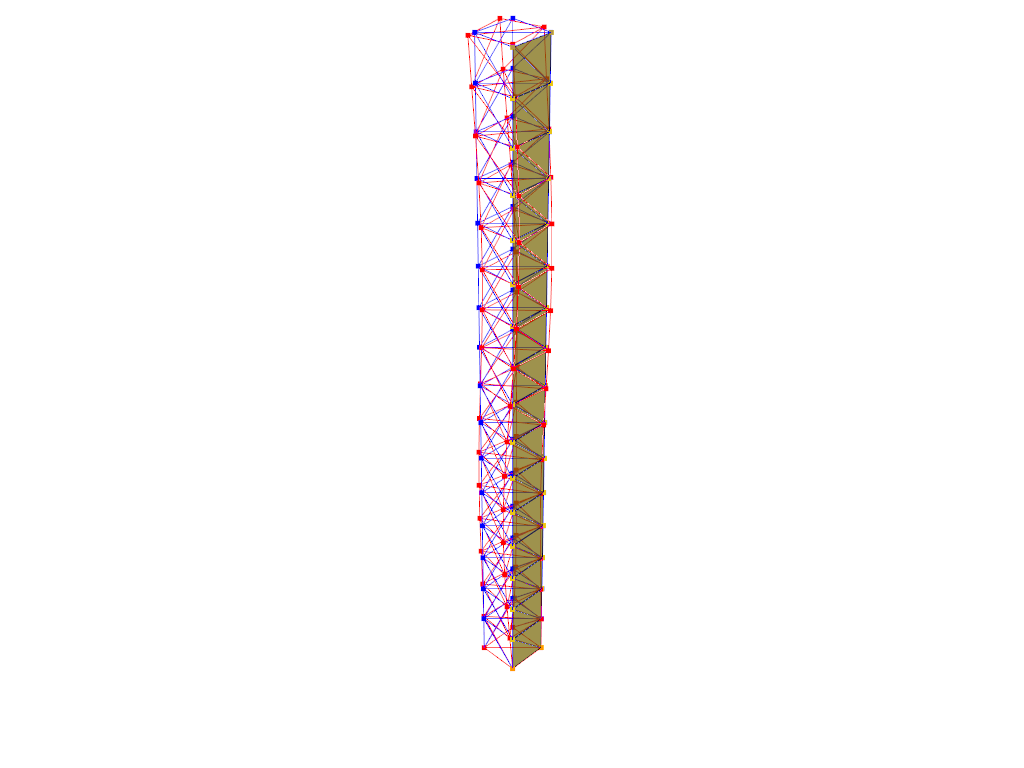
\includegraphics[width=\textwidth]{FOTOS/mod7_16.png}
        \caption{Séptimo modo de vibración N=16.}
    \end{minipage}
    \hfill
    \begin{minipage}[b]{0.5\textwidth}
        \centering
        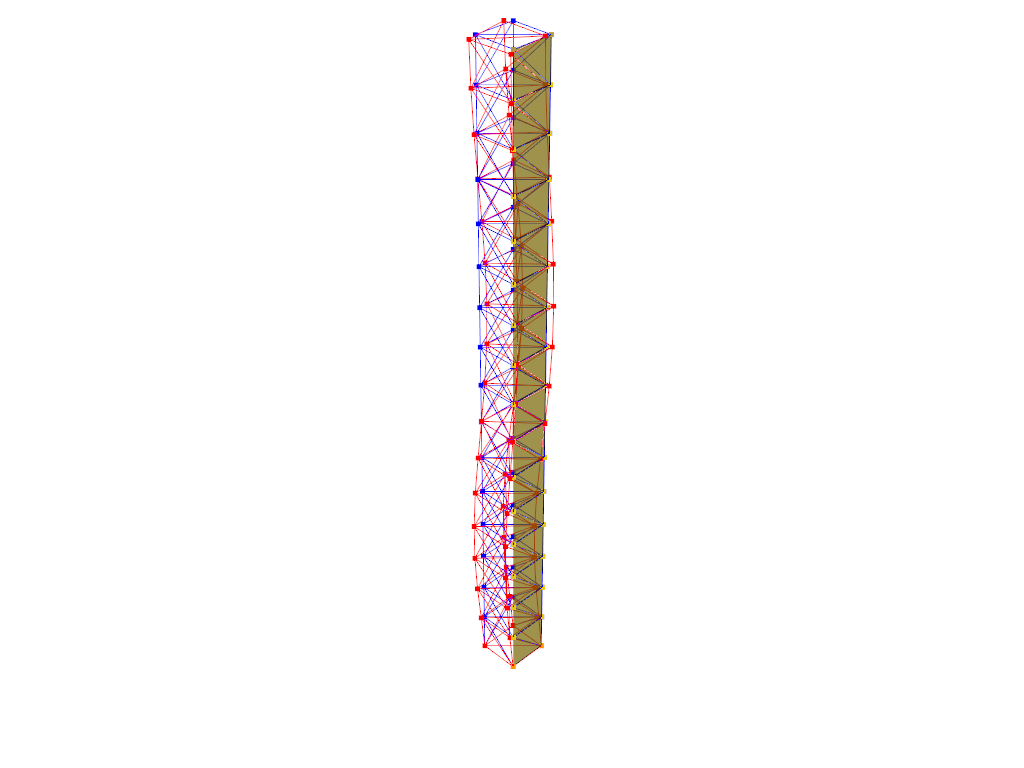
\includegraphics[width=\textwidth]{FOTOS/mod8_16.png}
        \caption{Octavo modo de vibración N=16.}
    \end{minipage}
\end{figure}

\begin{figure}[H]
    \begin{minipage}[b]{0.5\textwidth}
        \centering
        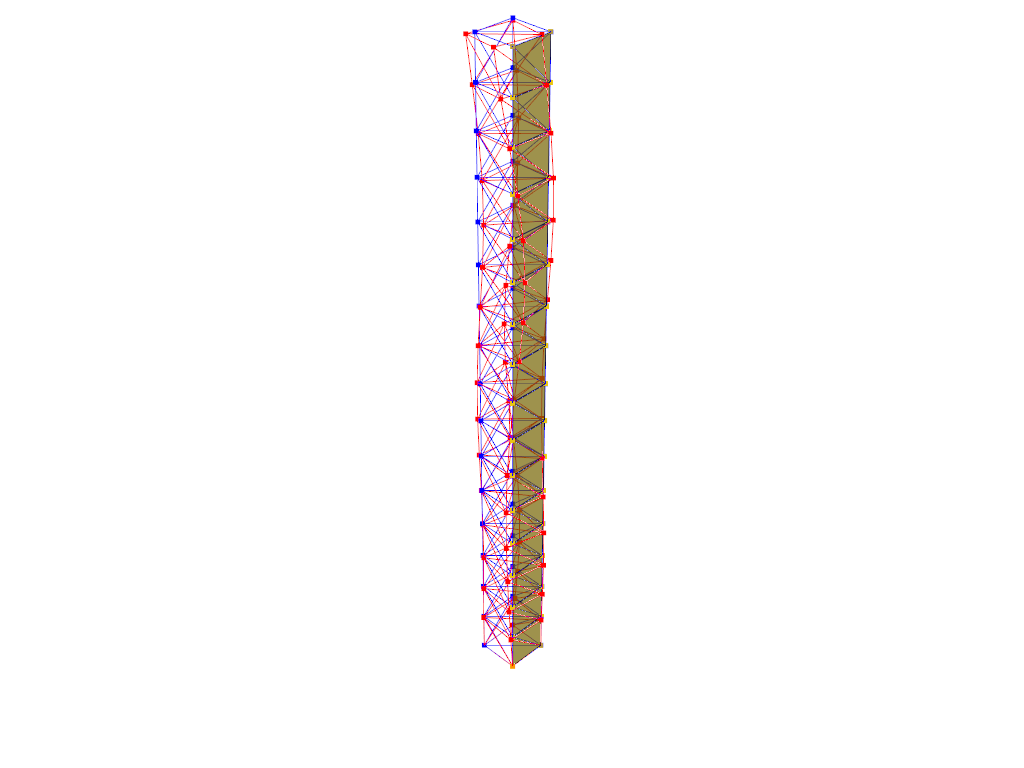
\includegraphics[width=\textwidth]{FOTOS/mod9_16.png}
        \caption{Noveno modo de vibración N=16.}
    \end{minipage}
    \hfill
    \begin{minipage}[b]{0.5\textwidth}
        \centering
        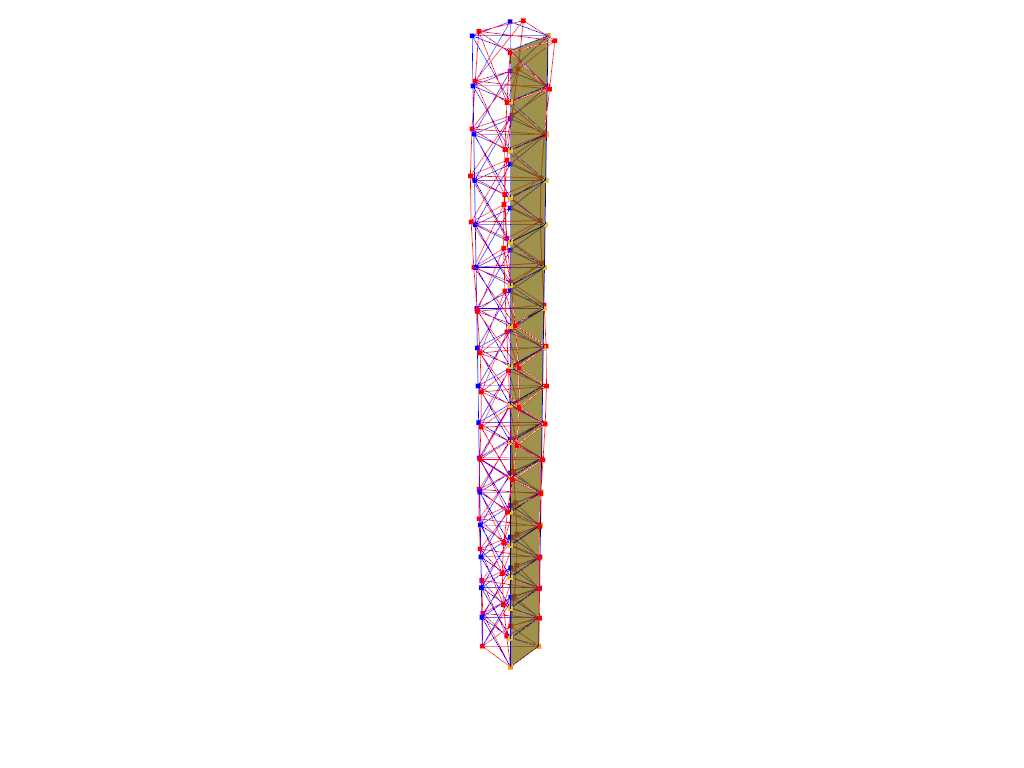
\includegraphics[width=\textwidth]{FOTOS/mod10_16.png}
        \caption{Décimo modo de vibración N=16.}
    \end{minipage}
\end{figure}

\subsection{Comparación de los casos}

En este caso, se puede observar que a medida que aumenta el número de vanos, las frecuencias de vibración disminuyen, para una misma sección transversal. Esto ocurre porque la estructura se vuelve más flexible al aumentar su longitud total, lo que genera una menor rigidez global, haciendo que las vibraciones sean más lentas.

En cuanto a distintas secciones transversales para un mismo N, las frecuencias aumentan con el área de la sección. Una sección transversal mayor aumenta la rigidez en cada vano, lo cual incrementa las frecuencias, porque la rigidez y la masa estructural determinan la resistencia a la vibración, es decir, estructuras más rígidas vibran a frecuencias más altas, mientras que las más dúctiles tienen frecuencias más bajas.

Por lo tanto, se puede decir que la estructura con mayor frecuencia es la del caso de 2 vanos con un porcentaje de RME del 30\%, y la de menor frecuencia es la del caso de 16 vanos con un porcentaje de RME del 10\%.

Además, cabe mencionar que no en todos los casos se logró la frecuencia fundamental mínima esperada de 0.1 Hz. En este caso, los que lograron la frecuencia fundamental mínima esperada fueron los casos de 2 y 4 vanos, mientras que los casos de 8 y 16 vanos no la lograron.

En el caso de que la estructura no fuese ``lineal'' la relación entre RME, cantidad de vanos y frecuencias de vibración no sería tan directa, ya que la distribución de cargas en los nodos no sería uniforme y la frecuencia dependería de la geometría del reticulado, junto con el RME. Luego, al ser superficial, podría ofrecer mayor rigidez y estabilidad, pero al aumentar los vanos el modo de vibrar de la estructura podría cambiar, generando zonas con concentraciones de tensiones y deformaciones, lo que podría afectar la vida útil de la estructura.

\newpage

\section{Conclusión}

En conclusión, el análisis del reticulado espacial fue exitoso. Se logró destacar cómo la frecuencia de vibración depende tanto de la cantidad de vanos como de la relación de masa estructural (RME). 

Así, estructuras más largas y flexibles (con mayor N) presentan frecuencias naturales menores, mientras que una sección transversal mayor aumenta la rigidez, al igual que las frecuencias de las estructuras. Con esto, se puede concluir que solo las configuraciones con 2 y 4 vanos cumplieron con la frecuencia mínima de 0.1 Hz.

En casos donde el diseño no es lineal, el comportamiento de las frecuencias es aún más complejo debido a la variabilidad en la distribución de tensiones y deformaciones. Esto puede influir en la durabilidad y estabilidad, generando zonas de concentración de esfuerzos. 


\part{Entrega 2}

\section{Introducción}

En este informe, se llevará a cabo un análisis estructural de un enrejado de la entrega 1, considerando la sección transversal más grande estudiada (\(A_{30}\)). Se evaluarán dos configuraciones posibles para el enrejado: una con una diagonal en cada cara y otra con dos diagonales cruzadas en las caras laterales e interiores. El objetivo es analizar cómo las deformaciones y las fuerzas axiales de las barras se comportan bajo diferentes condiciones de carga, específicamente con una aceleración de 0.1g en los tres ejes y un aumento de temperatura de 100°C en los nodos.

El análisis se dividirá en dos partes. En la primera, se analizarán las deformaciones y las fuerzas axiales en función de las condiciones de aceleración y temperatura, mostrando las deformaciones y la distribución de las fuerzas axiales para cada caso. En la segunda parte, se estudiará la "peor dirección" de aceleración, entendida como la dirección en la que se maximiza o minimiza la carga axial en las barras, considerando que la aceleración puede ser en cualquier dirección en el espacio 3D.

\section{Resultados}

\subsection{Parte 1}

Para esta sección se seleccionó un reticulado de 16 vanos para una mejor visualización de los resultados. A este, se le realizaron análisis de deformación y esfuerzos internos frente a aceleraciones aplicadas en cada dirección $x$, $y$, $z$. Posteriormente, se compararon y obtuvieron los resultados pertinentes.

\subsubsection{Aceleración en Eje X}

\begin{figure}[H]
    \centering
    \begin{minipage}{0.45\textwidth}
        \centering
        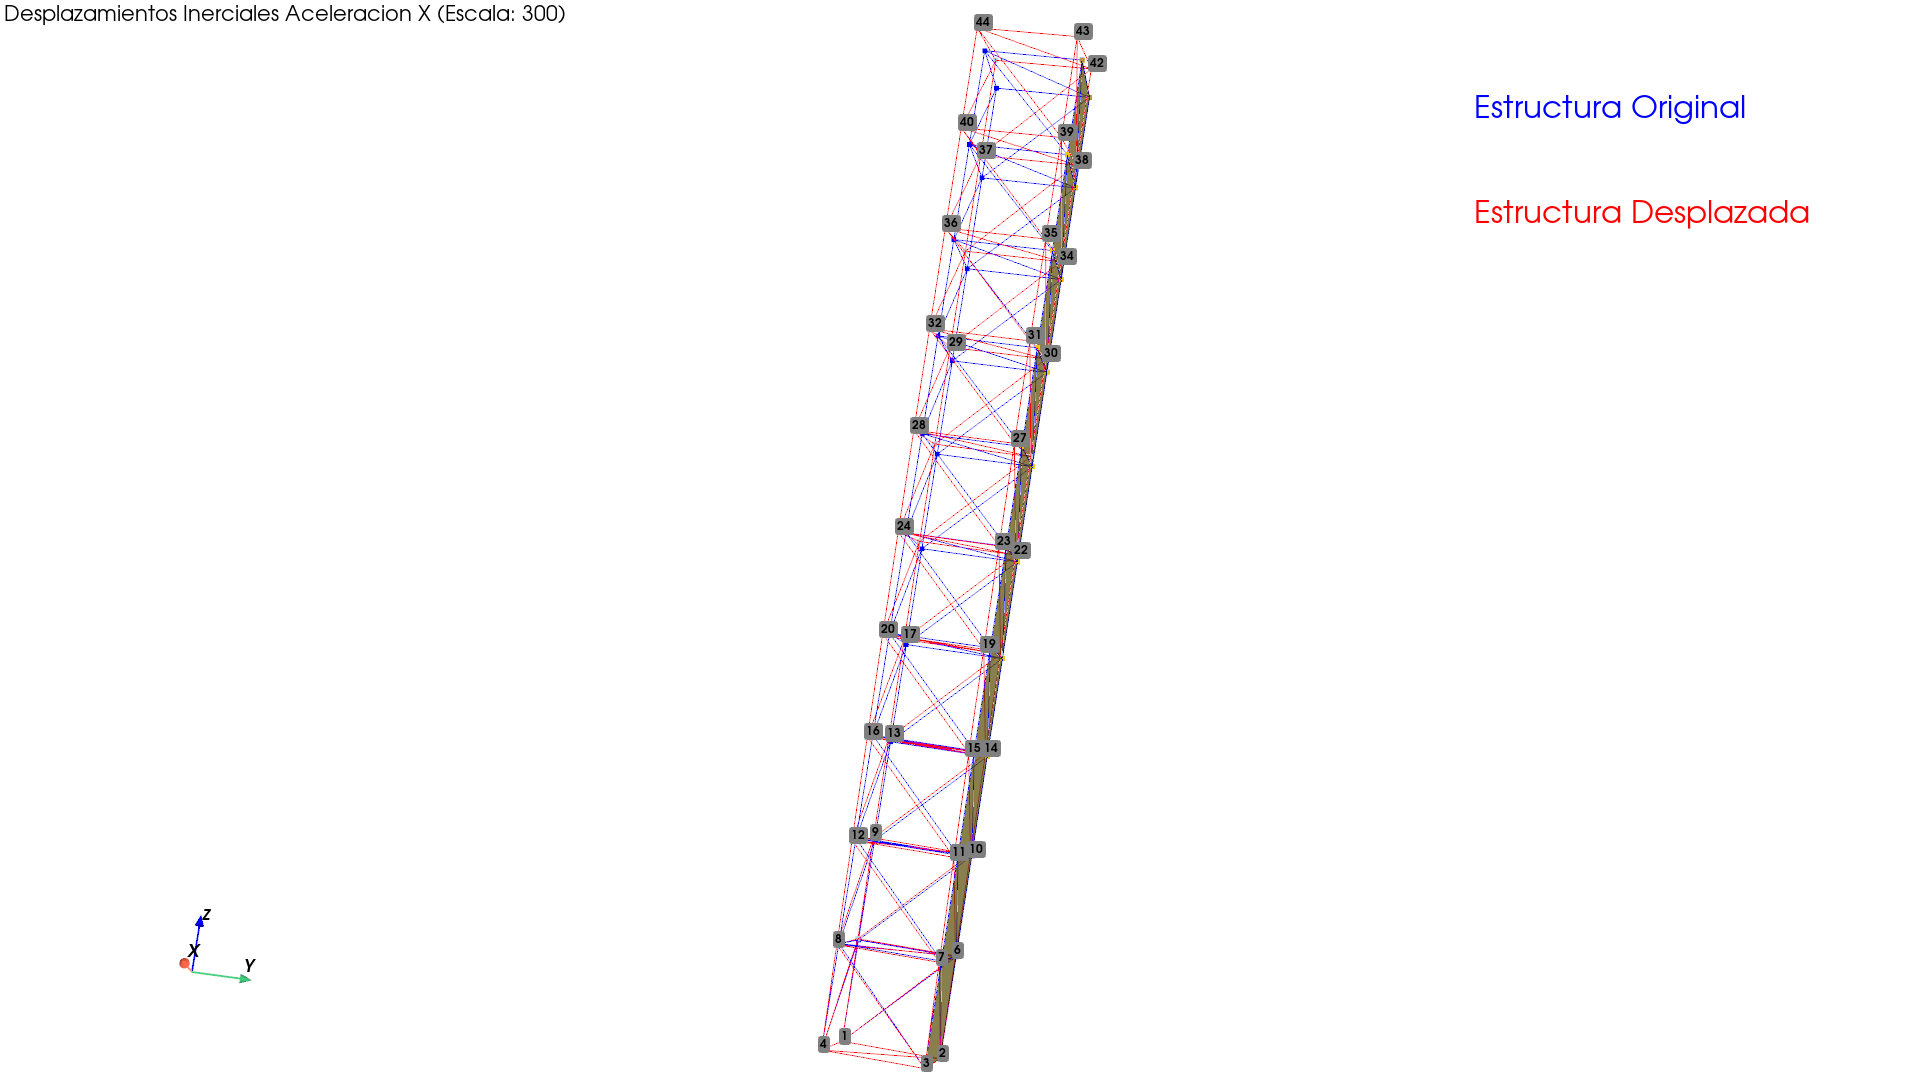
\includegraphics[width=\textwidth]{GRAFICOS/Desplazamientos Inerciales Aceleracion X False.png}
        \caption{Desplazamiento en X estructura sin diagonales cruzadas.}
        \label{fig:imagen1}
    \end{minipage}
    \hfill
    \begin{minipage}{0.45\textwidth}
        \centering
        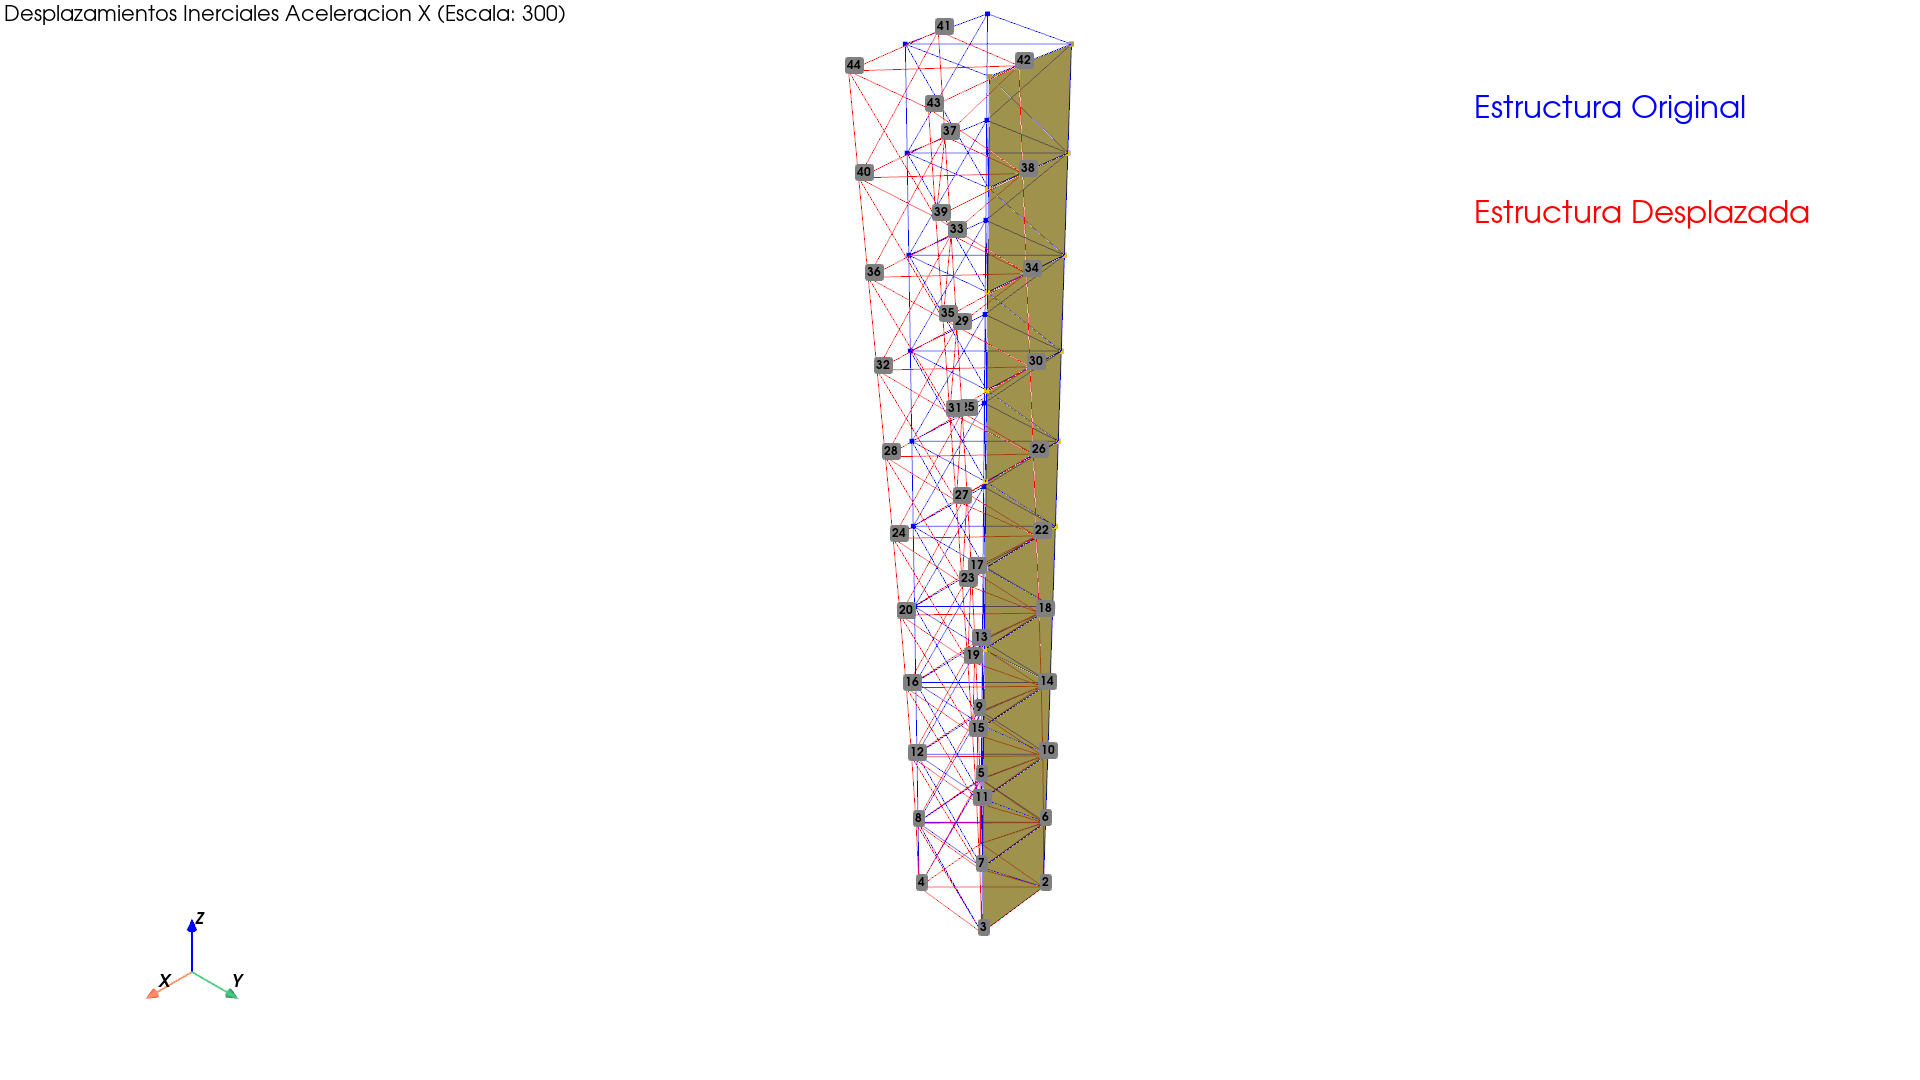
\includegraphics[width=\textwidth]{GRAFICOS/Desplazamientos Inerciales Aceleracion X True.png}
        \caption{Desplazamiento en X estructura con diagonales cruzadas.}
        \label{fig:imagen2}
    \end{minipage}
\end{figure}

\begin{figure}[H]
    \centering
    \begin{minipage}{0.45\textwidth}
        \centering
        \includegraphics[width=\textwidth]{GRAFICOS/Esfuerzos Internos Máximos en las Barras Aceleracion X False.png}
        \caption{Esfuerzos internos en estructura sin diagonales cruzadas.}
        \label{fig:imagen11}
    \end{minipage}
    \hfill
    \begin{minipage}{0.45\textwidth}
        \centering
        \includegraphics[width=\textwidth]{GRAFICOS/Esfuerzos Internos Máximos en las Barras Aceleracion X True.png}
        \caption{Esfuerzos internos en estructura con diagonales cruzadas.}
        \label{fig:imagen22}
    \end{minipage}
\end{figure}

\subsubsection{Aceleración en Eje Y}

\begin{figure}[H]
    \centering
    \begin{minipage}{0.45\textwidth}
        \centering
        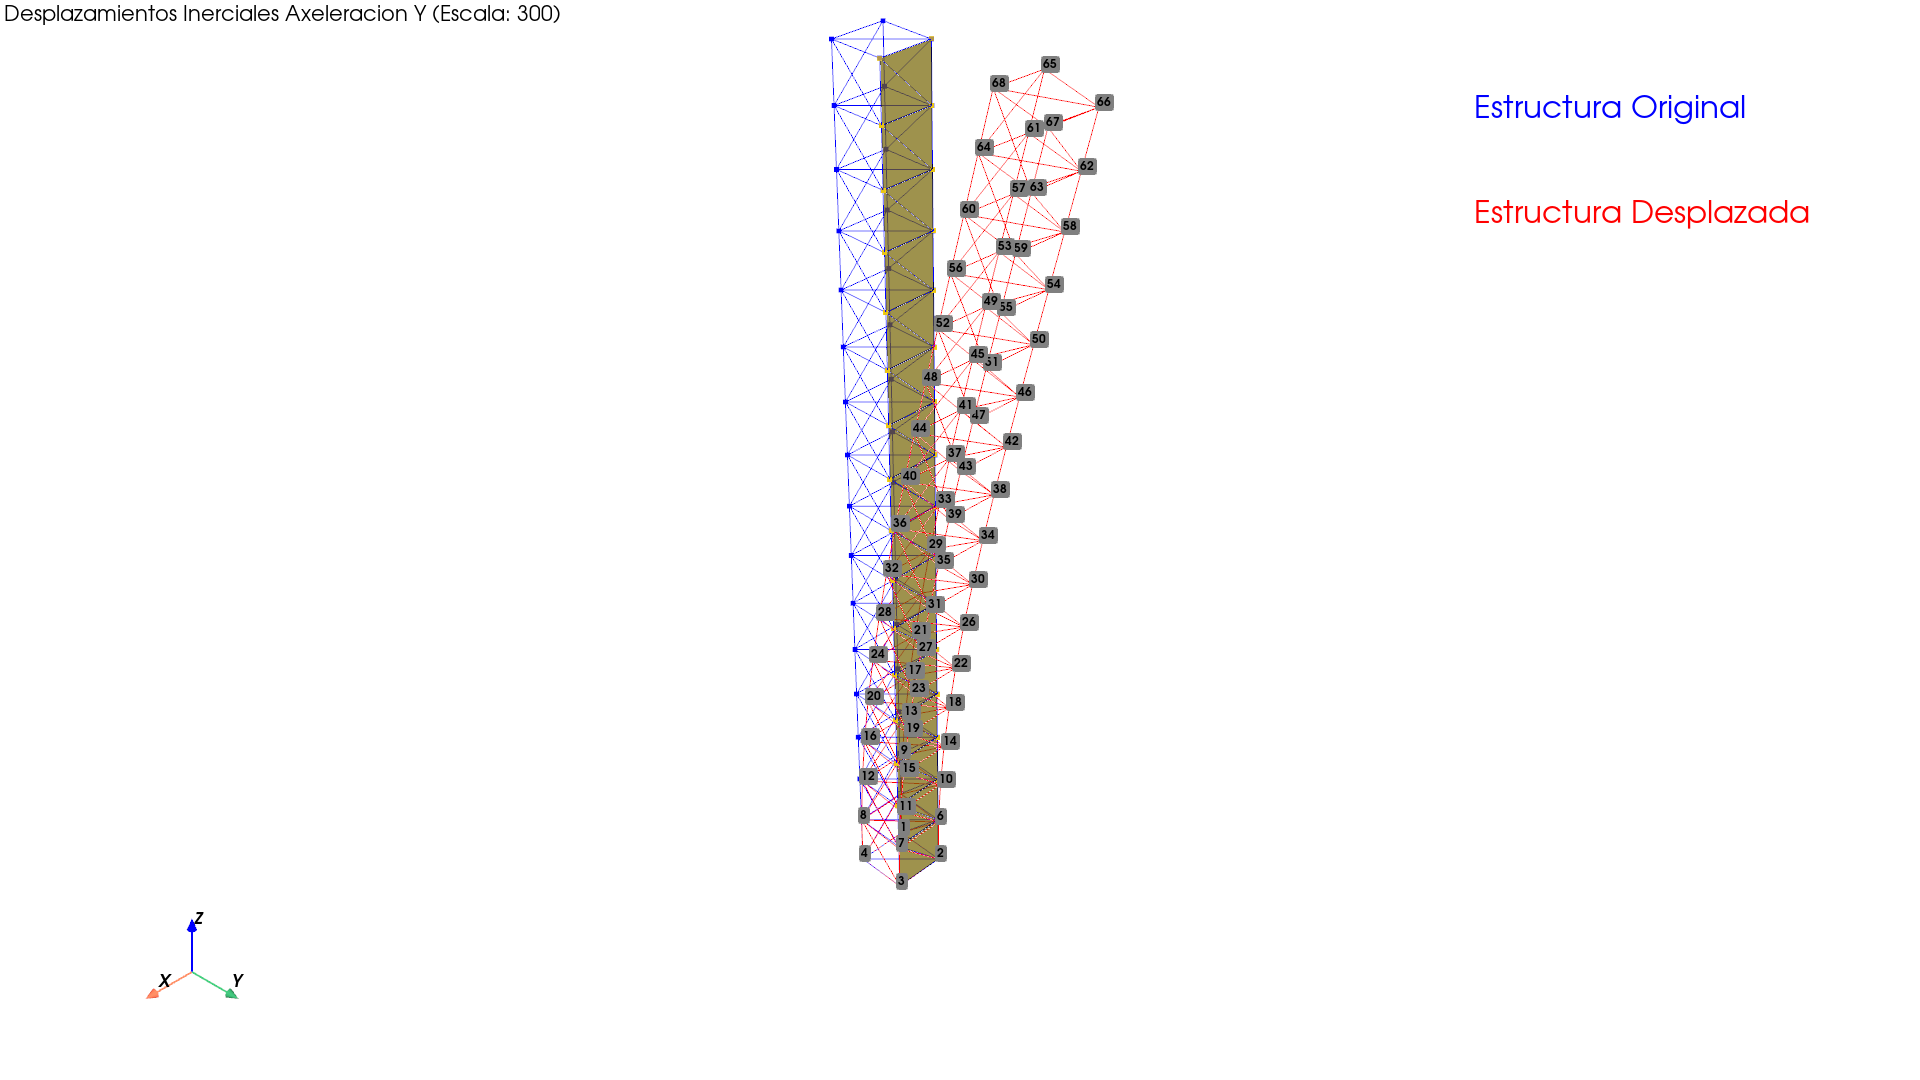
\includegraphics[width=\textwidth]{GRAFICOS/Desplazamientos Inerciales Axeleracion Y False.png}
        \caption{Desplazamiento en Y estructura sin diagonales cruzadas.}
        \label{fig:imagen3}
    \end{minipage}
    \hfill
    \begin{minipage}{0.45\textwidth}
        \centering
        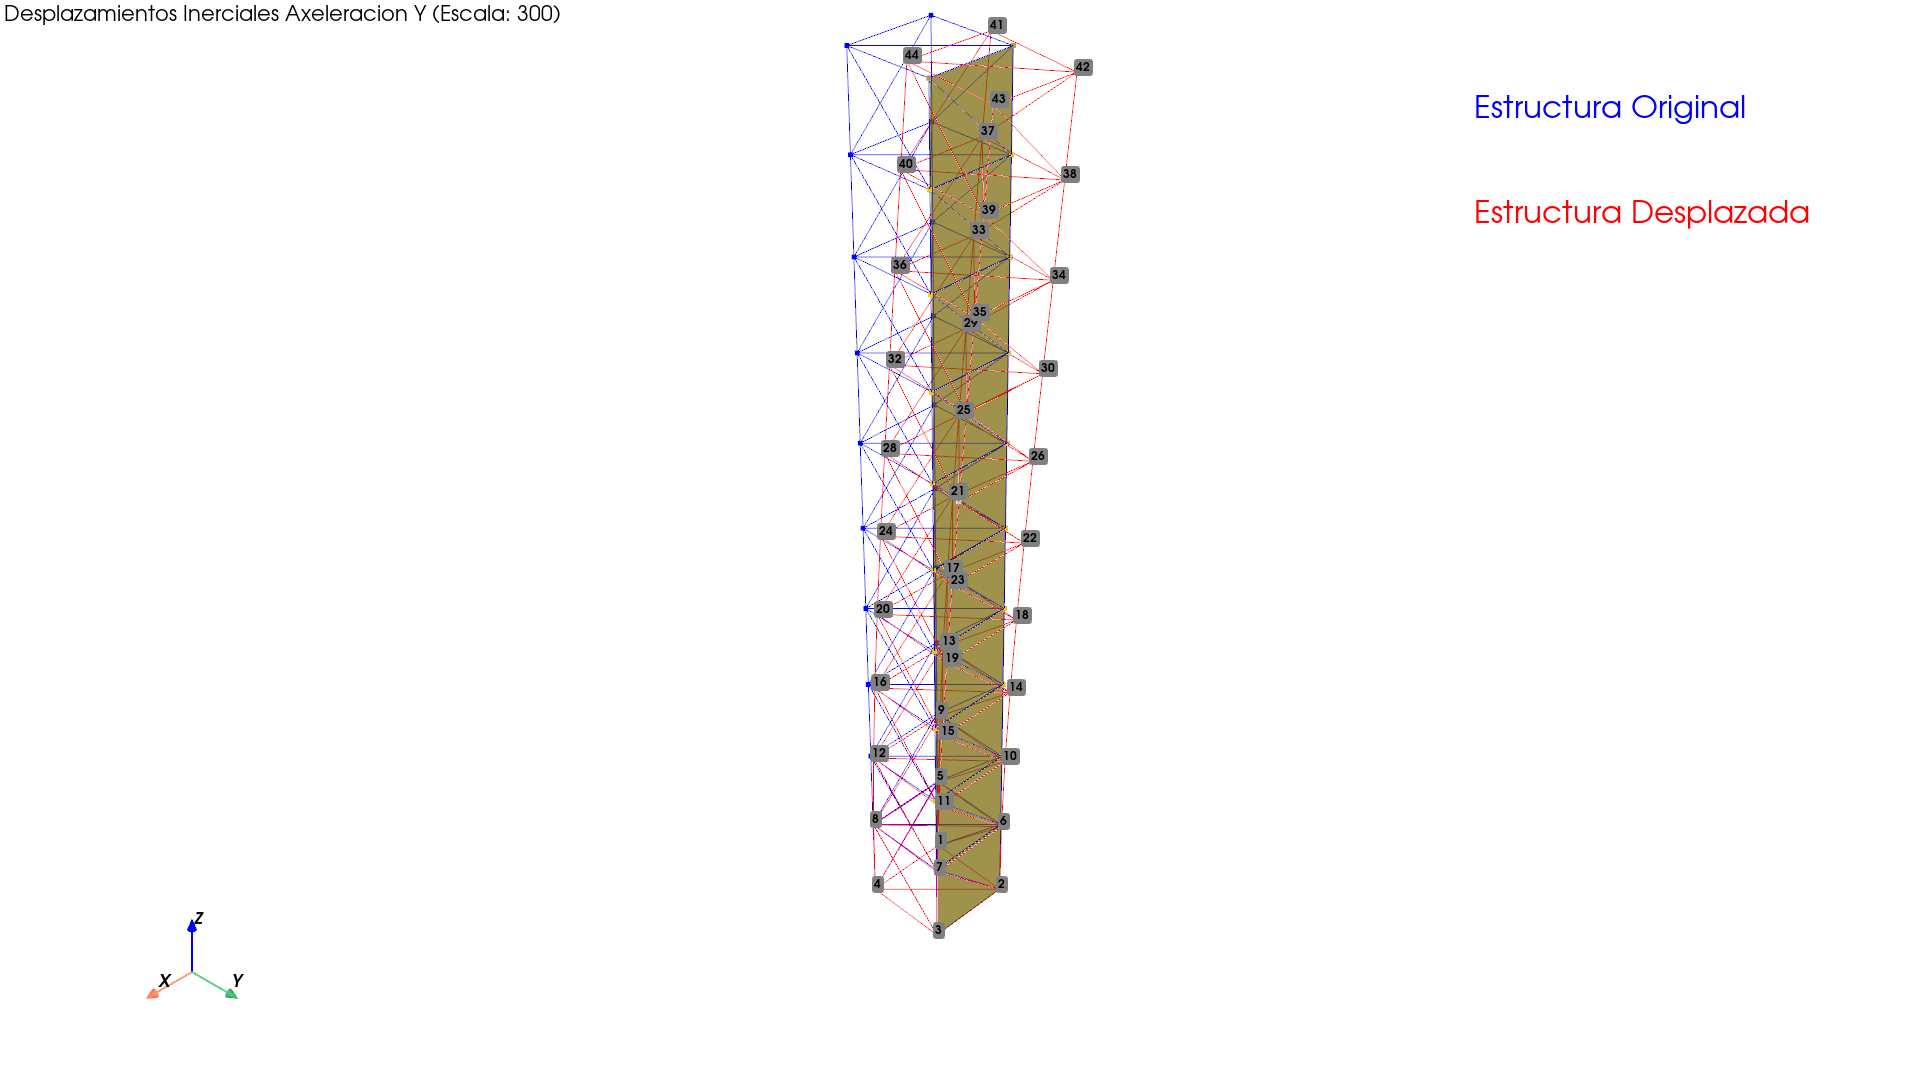
\includegraphics[width=\textwidth]{GRAFICOS/Desplazamientos Inerciales Axeleracion Y True.png}
        \caption{Desplazamiento en Y estructura con diagonales cruzadas.}
        \label{fig:imagen4}
    \end{minipage}
\end{figure}

\begin{figure}[H]
    \centering
    \begin{minipage}{0.45\textwidth}
        \centering
        \includegraphics[width=\textwidth]{GRAFICOS/Esfuerzos Internos Máximos en las Barras Axeleracion Y False.png}
        \caption{Esfuerzos internos en estructura sin diagonales cruzadas.}
        \label{fig:imagen33}
    \end{minipage}
    \hfill
    \begin{minipage}{0.45\textwidth}
        \centering
        \includegraphics[width=\textwidth]{GRAFICOS/Esfuerzos Internos Máximos en las Barras Axeleracion Y True.png}
        \caption{Esfuerzos internos en estructura con diagonales cruzadas.}
        \label{fig:imagen44}
    \end{minipage}
\end{figure}

\subsubsection{Aceleración en Eje Z}

\begin{figure}[H]
    \centering
    \begin{minipage}{0.45\textwidth}
        \centering
        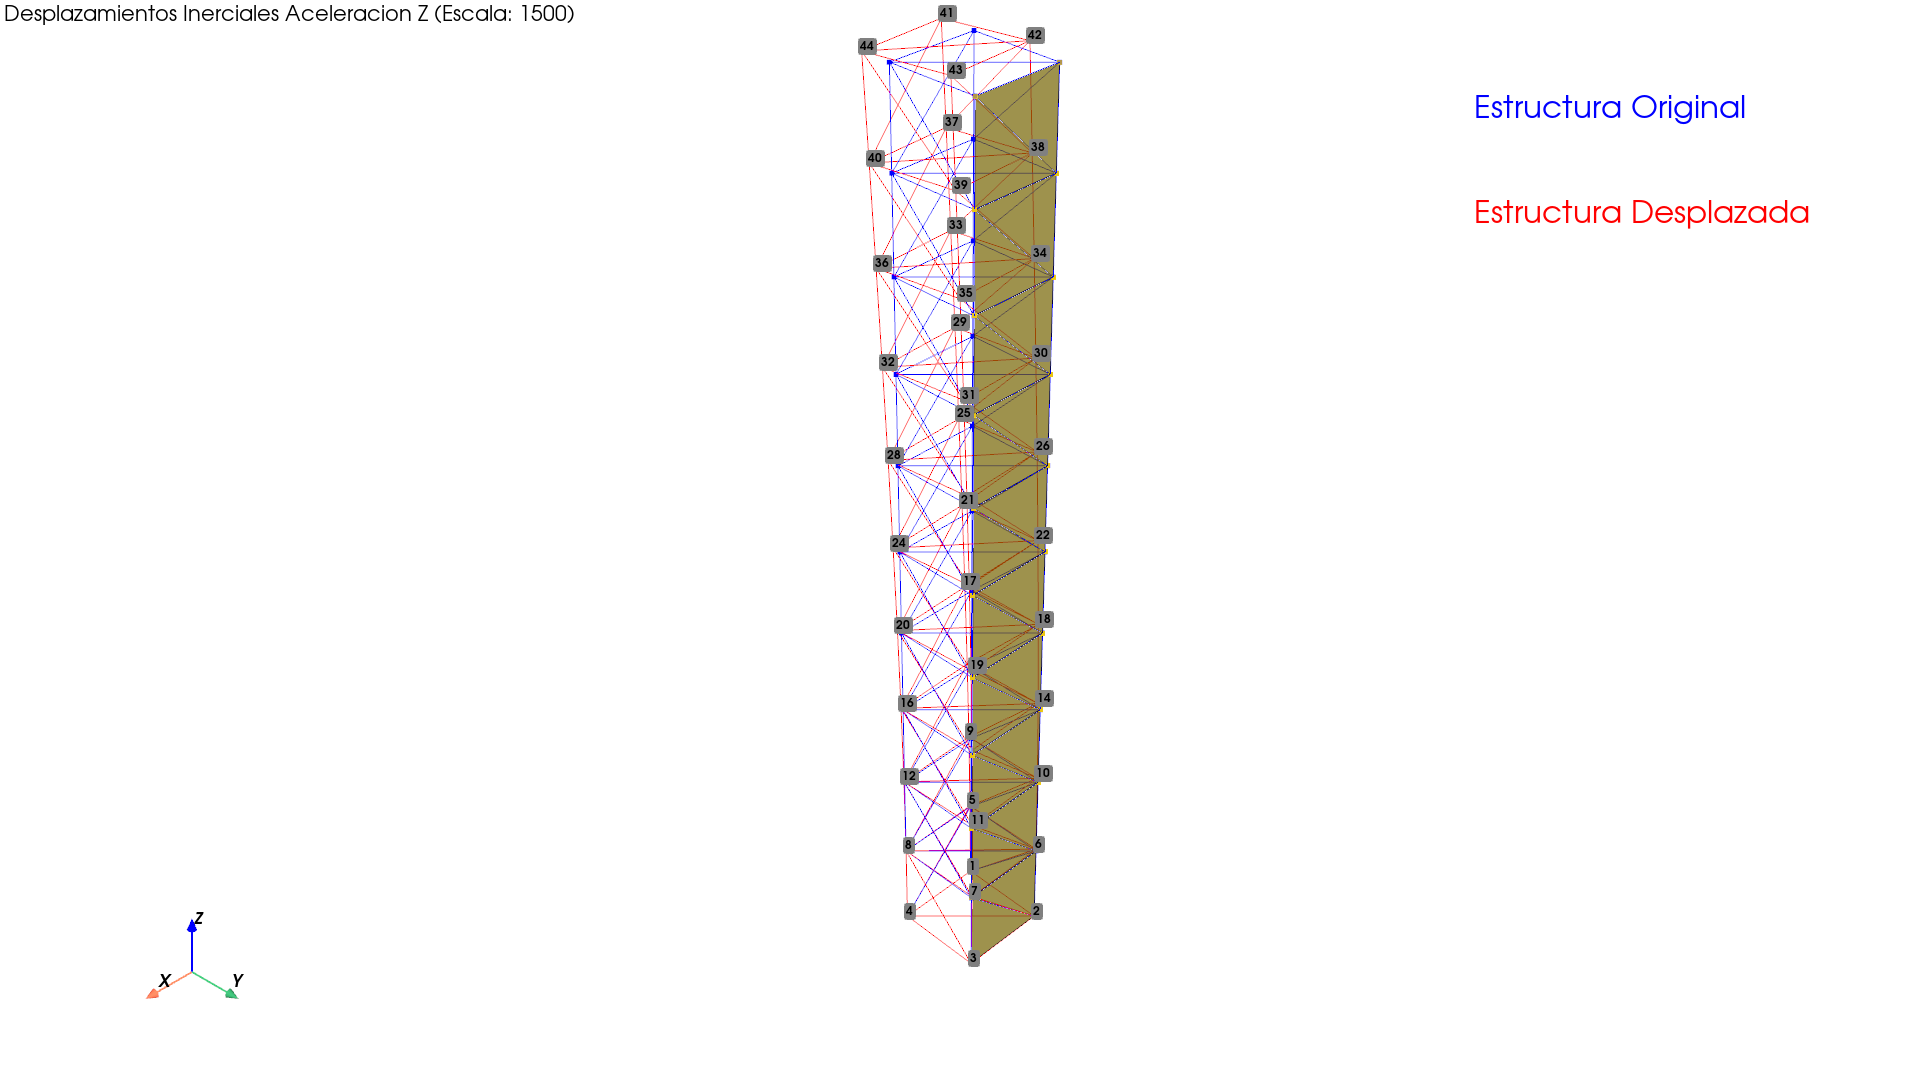
\includegraphics[width=\textwidth]{GRAFICOS/Desplazamientos Inerciales Aceleracion Z False.png}
        \caption{Desplazamiento en Z estructura sin diagonales cruzadas.}
        \label{fig:imagen5}
    \end{minipage}
    \hfill
    \begin{minipage}{0.45\textwidth}
        \centering
        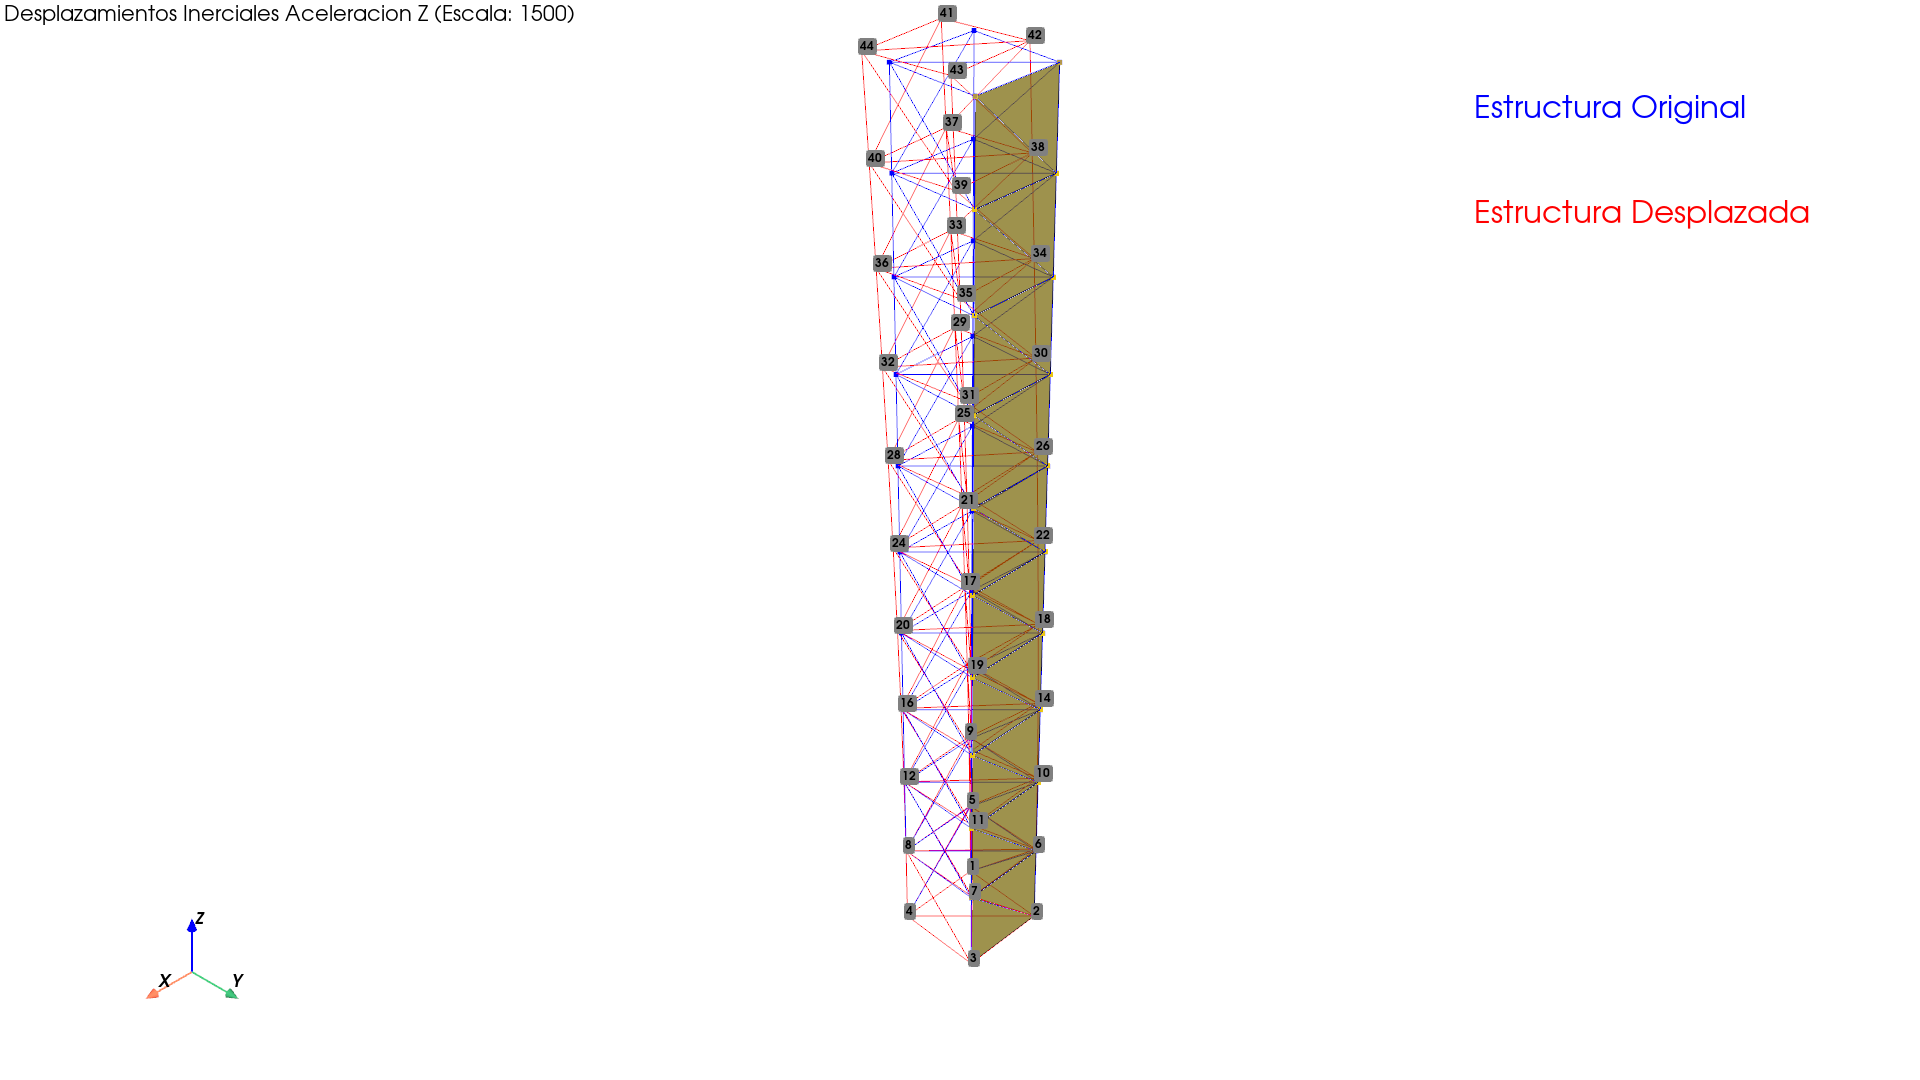
\includegraphics[width=\textwidth]{GRAFICOS/Desplazamientos Inerciales Aceleracion Z True.png}
        \caption{Desplazamiento en Z estructura con diagonales cruzadas.}
        \label{fig:imagen6}
    \end{minipage}
\end{figure}

\begin{figure}[H]
    \centering
    \begin{minipage}{0.45\textwidth}
        \centering
        \includegraphics[width=\textwidth]{GRAFICOS/Esfuerzos Internos Máximos en las Barras Aceleracion Z False.png}
        \caption{Esfuerzos internos en estructura sin diagonales cruzadas.}
        \label{fig:imagen55}
    \end{minipage}
    \hfill
    \begin{minipage}{0.45\textwidth}
        \centering
        \includegraphics[width=\textwidth]{GRAFICOS/Esfuerzos Internos Máximos en las Barras Aceleracion Z True.png}
        \caption{Esfuerzos internos en estructura con diagonales cruzadas.}
        \label{fig:imagen66}
    \end{minipage}
\end{figure}

\subsubsection{Aumento de temperatura en 100°C en nodos conectados al panel}

\begin{figure}[H]
    \centering
    \begin{minipage}{0.45\textwidth}
        \centering
        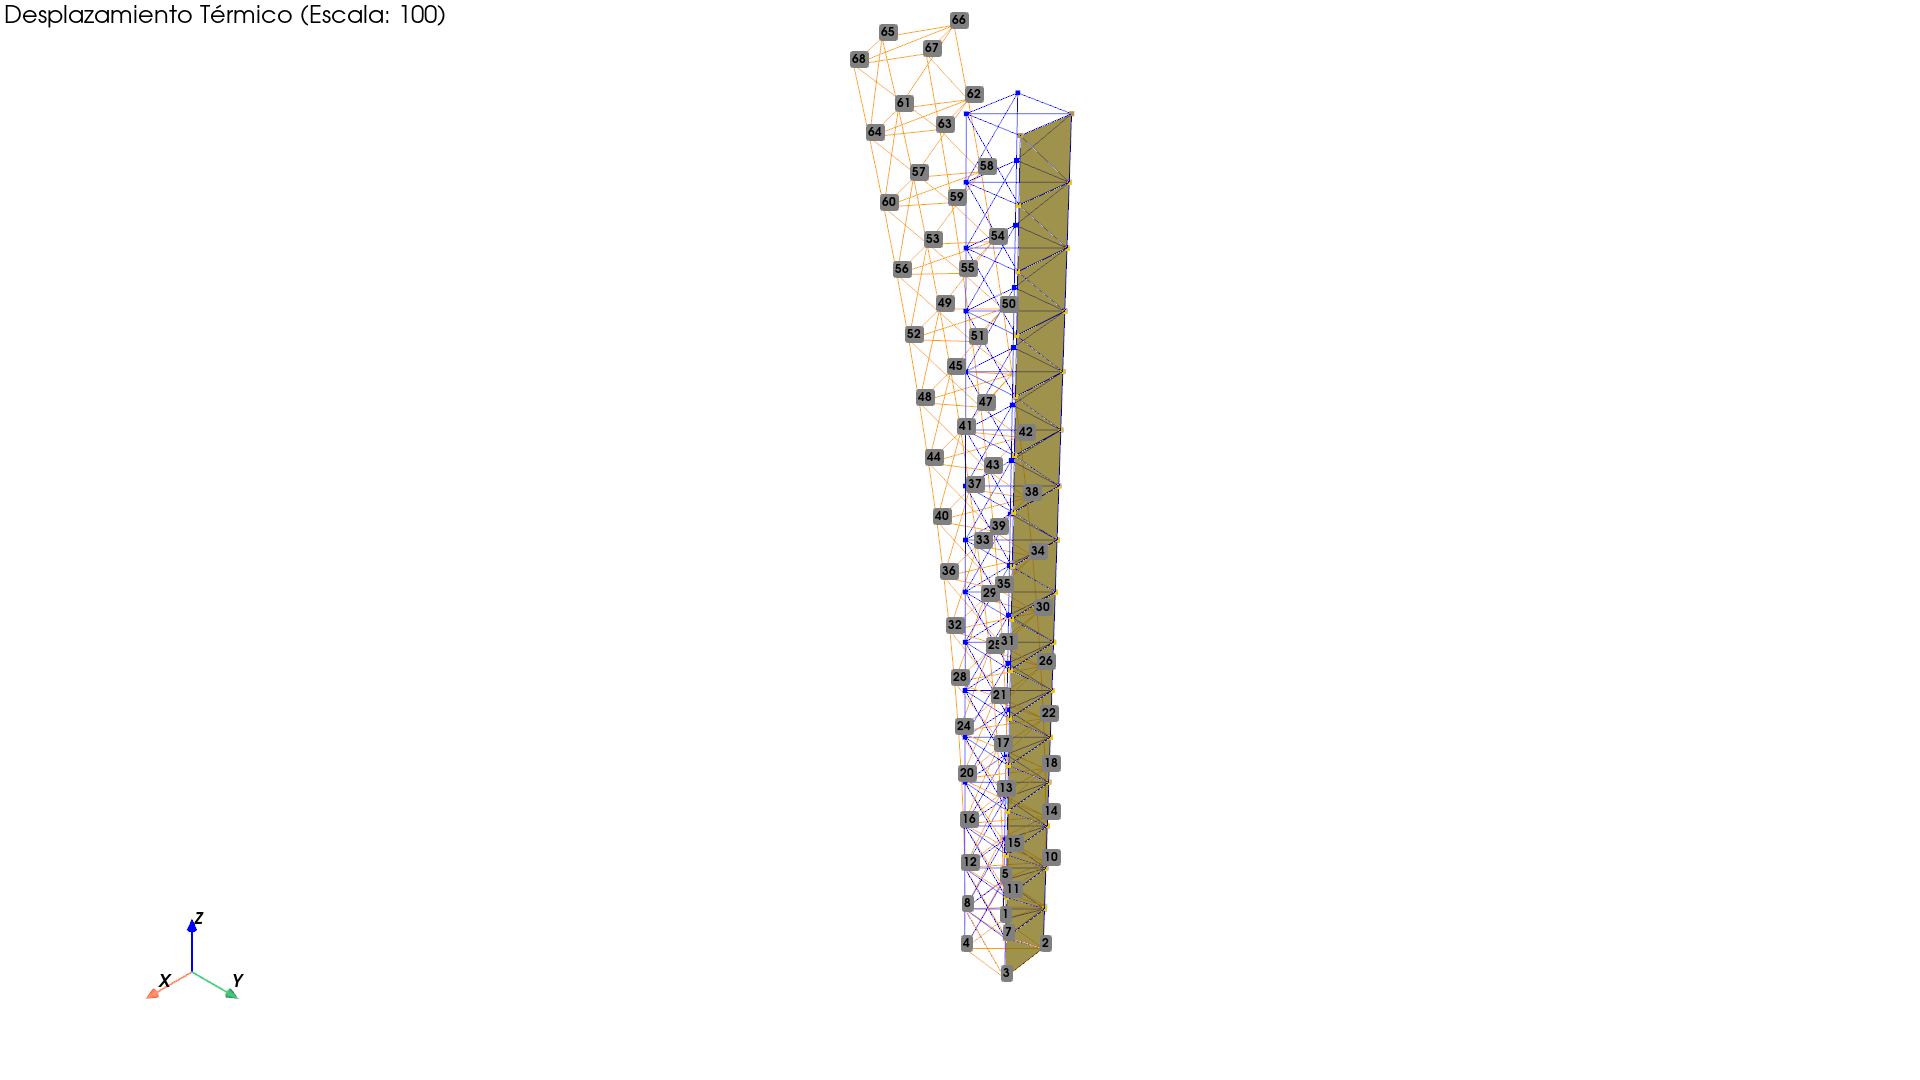
\includegraphics[width=\textwidth]{GRAFICOS/Desplazamientos Termicos False.png}
        \caption{Desplazamiento $\Delta T$ en estructura sin diagonales cruzadas.}
        \label{fig:imagen7}
    \end{minipage}
    \hfill
    \begin{minipage}{0.45\textwidth}
        \centering
        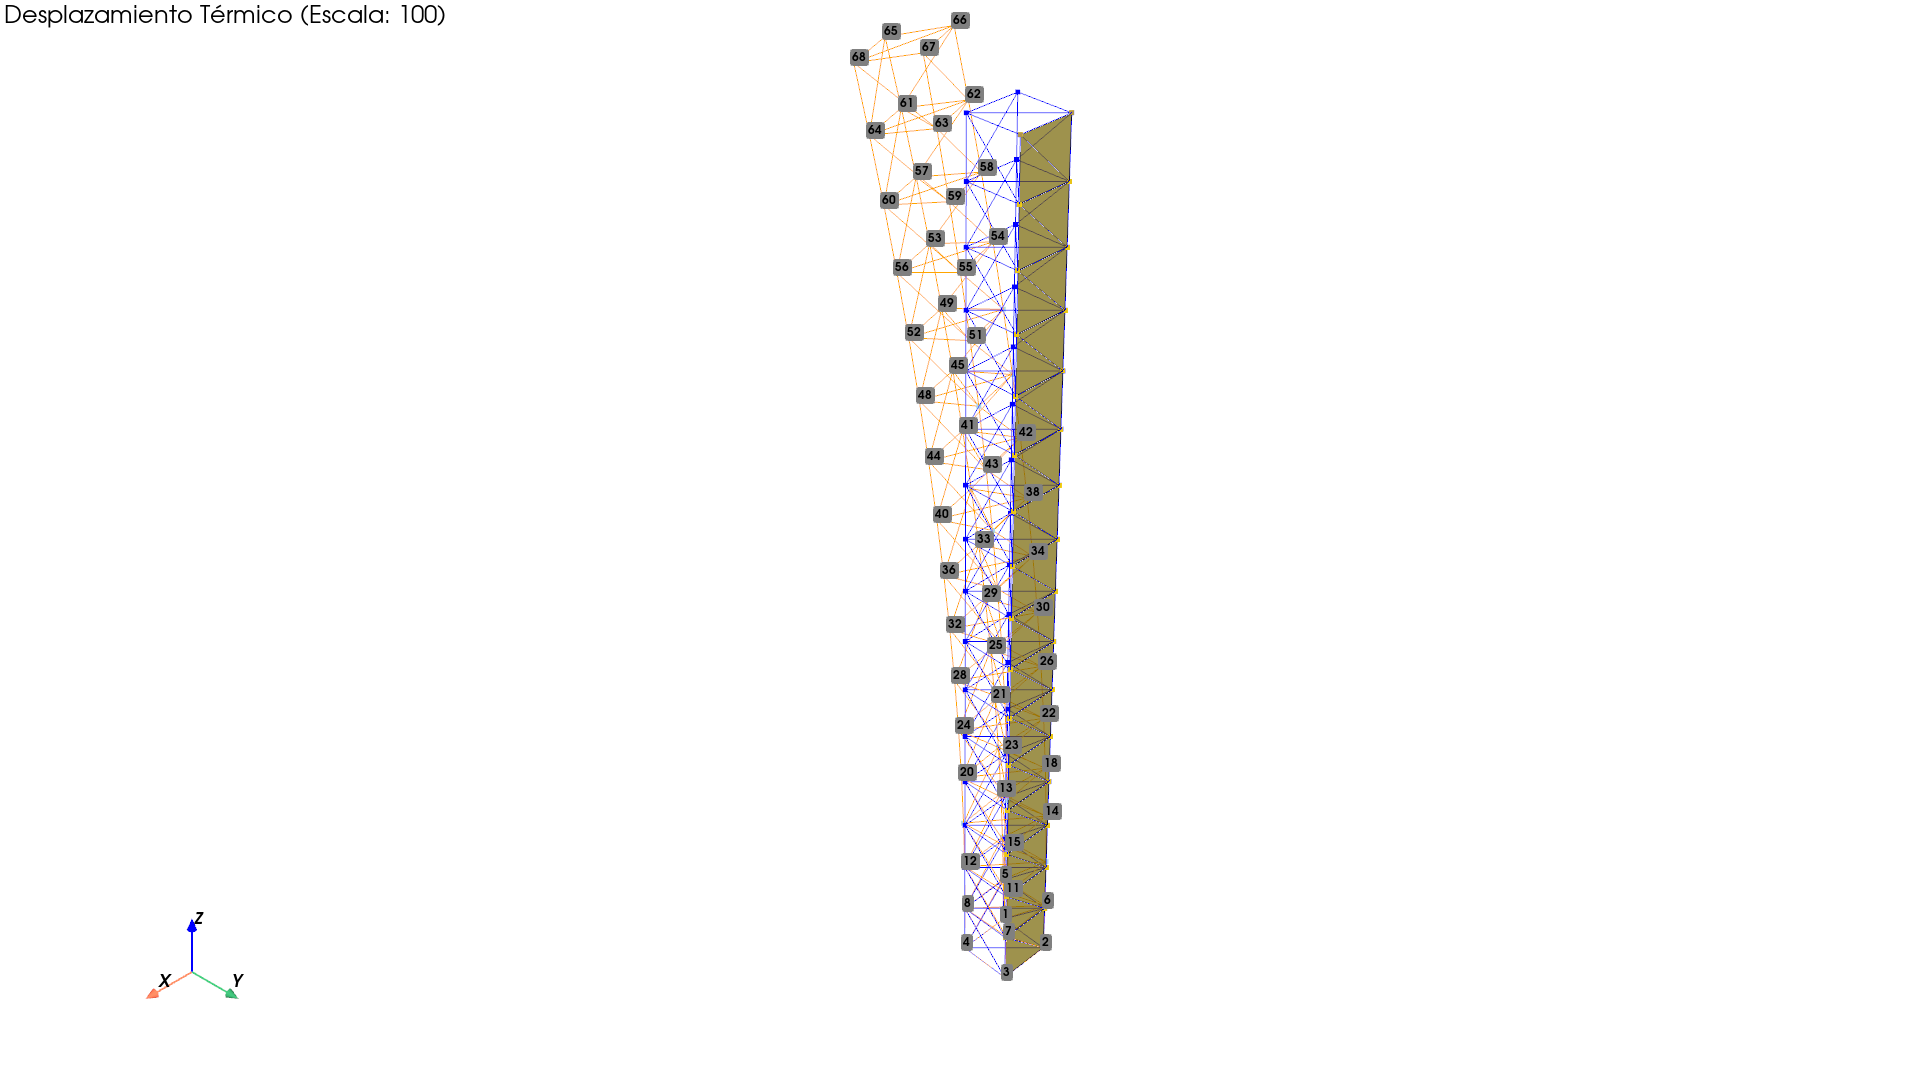
\includegraphics[width=\textwidth]{GRAFICOS/Desplazamientos Termicos True.png}
        \caption{Desplazamiento $\Delta T$ en estructura con diagonales cruzadas.}
        \label{fig:imagen8}
    \end{minipage}
\end{figure}

\begin{figure}[H]
    \centering
    \begin{minipage}{0.45\textwidth}
        \centering
        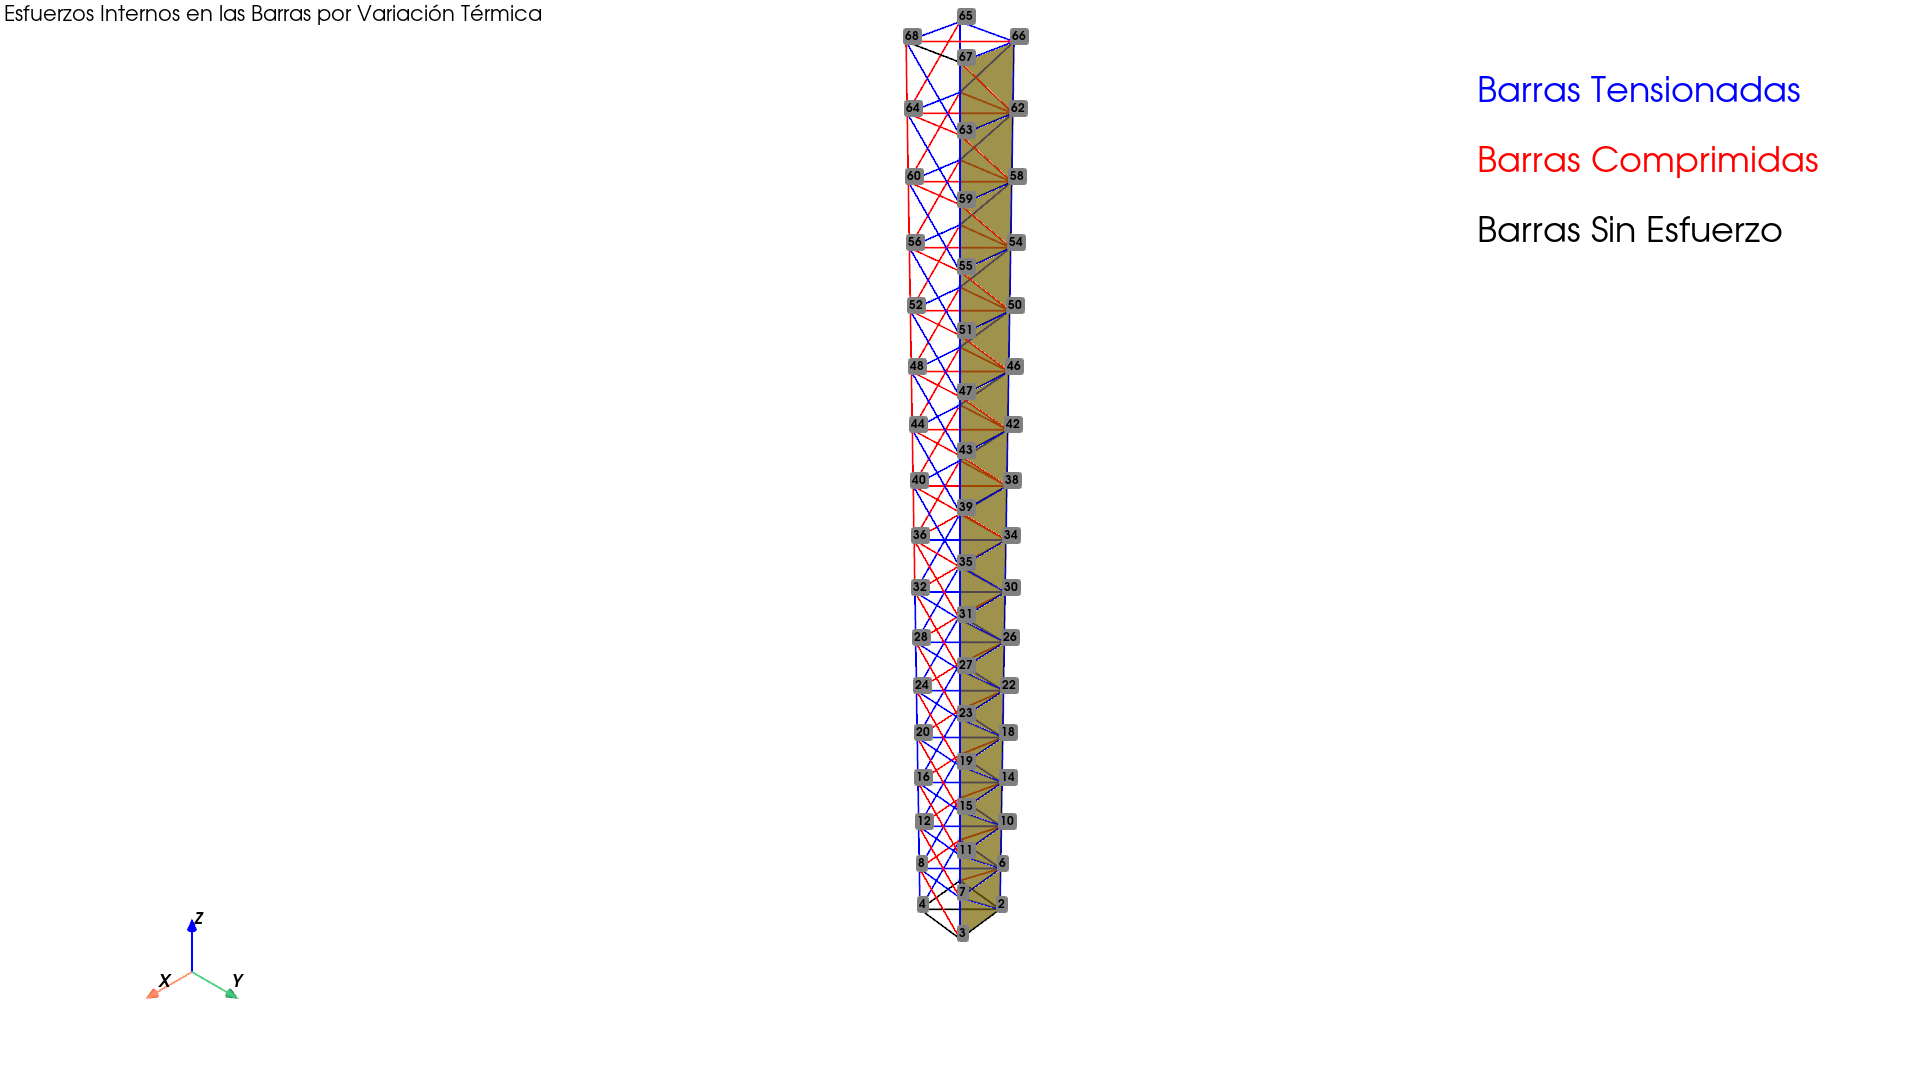
\includegraphics[width=\textwidth]{GRAFICOS/Esfuerzos Internos en las Barras por Variación Térmica False.png}
        \caption{Esfuerzos internos por $\Delta T$ en estructura sin diagonales cruzadas.}
        \label{fig:imagen77}
    \end{minipage}
    \hfill
    \begin{minipage}{0.45\textwidth}
        \centering
        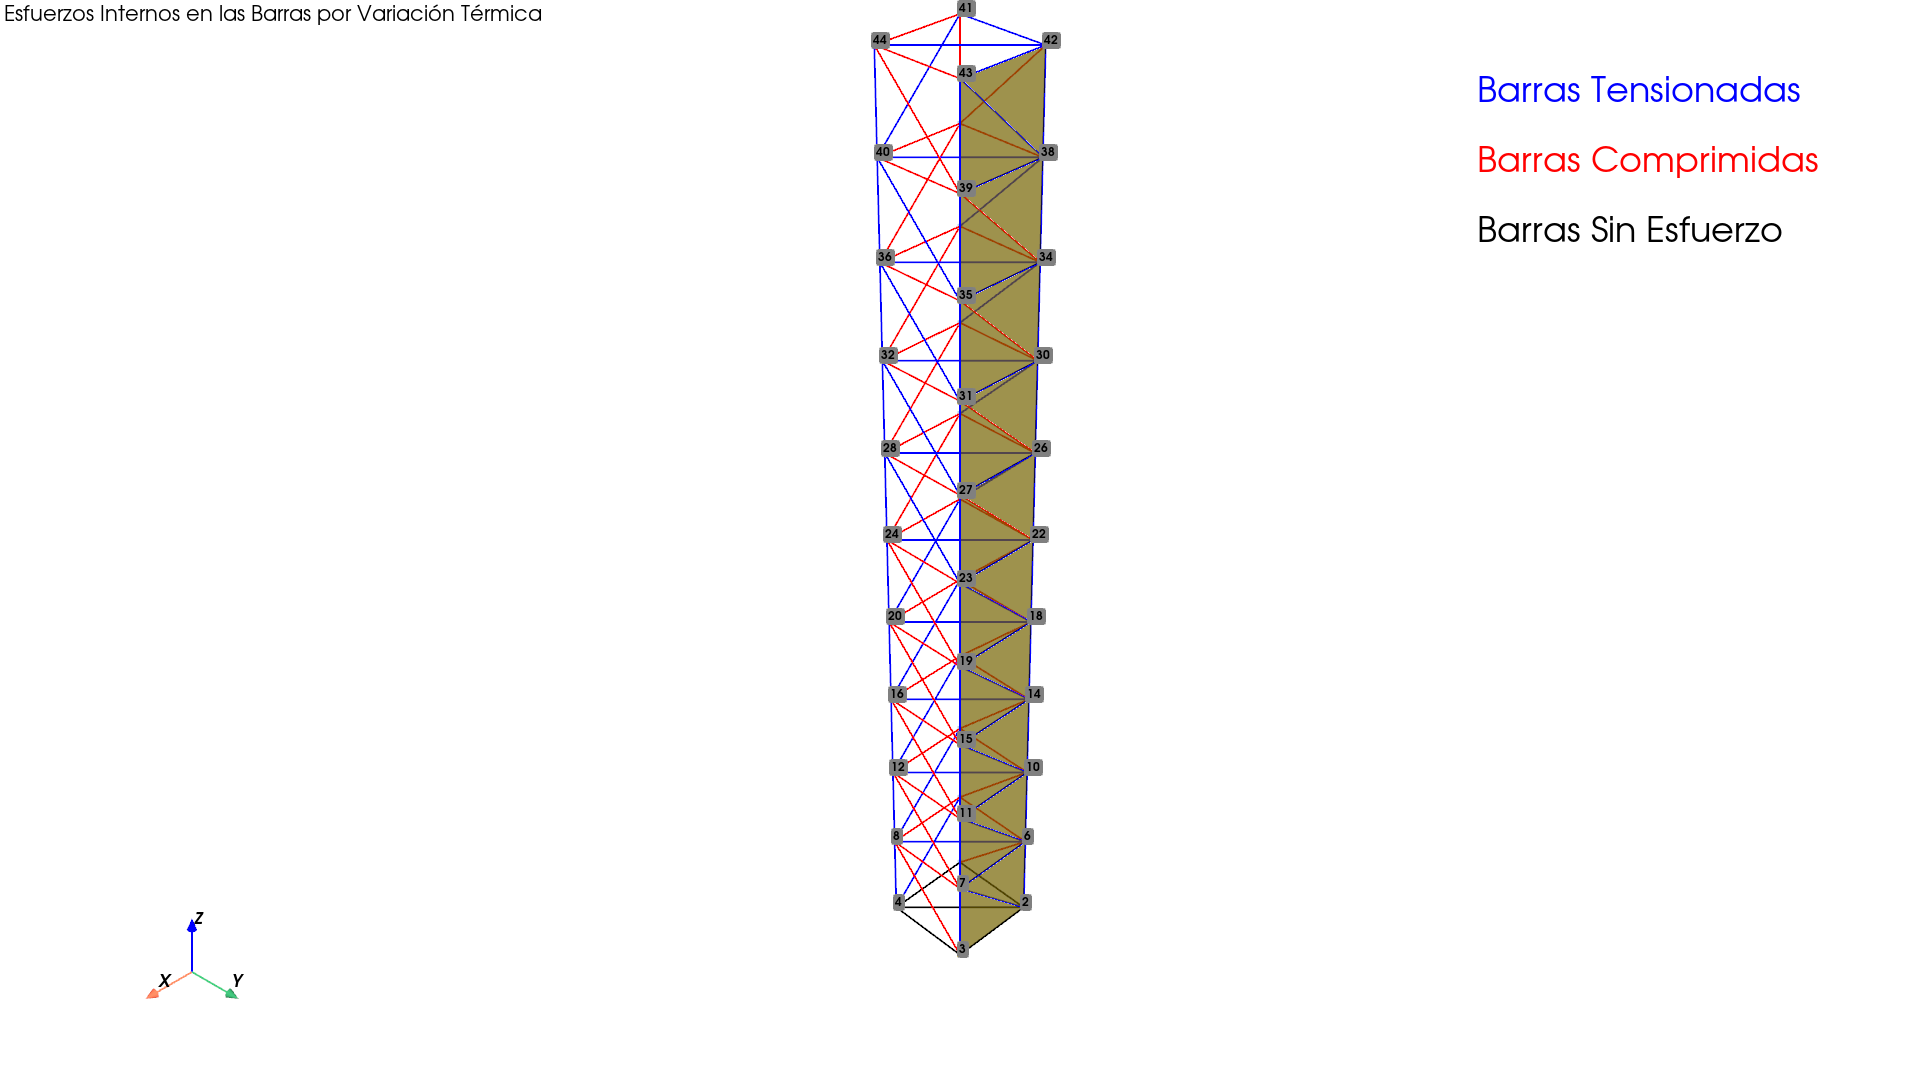
\includegraphics[width=\textwidth]{GRAFICOS/Esfuerzos Internos en las Barras por Variación Térmica True.png}
        \caption{Esfuerzos internos por $\Delta T$ en estructura con diagonales cruzadas.}
        \label{fig:imagen88}
    \end{minipage}
\end{figure}

Analizando y comparando cada imagen de deformaciones y tensiones en las direcciones X, Y, Z, se pueden obtener los siguientes resultados y observaciones.

En la imagen de desplazamiento inercial en la dirección X, la estructura muestra una deformación en la misma, desplazándose lateralmente.El mayor desplazamiento se observa en la parte superior, indicando que los elementos superiores son los más afectados frente a un cambio en su inercia. Los esfuerzos internos en las barras para esta dirección presentan barras comprimidas (de color rojo) en un lado y tensionadas (azules) en el lado opuesto, debido a la flexión inducida por la aceleración en X, las barras en diagonal muestran soportar los esfuerzos de tracción, mientras que la disposición cuadrada soporta los de compresión.

En la dirección Y, el comportamiento es similar al de la dirección X. Sin embargo, las barras en diagonal son las que soportan la mayor cantidad de esfuerzos de compresión, mientras que las cuadradas soportan los de tracción.

Por otro lado, la aceleración en Z provoca desplazamientos verticales en la estructura, con un patrón de deformación más simétrico en comparación con las direcciones X e Y. Los esfuerzos internos en las barras bajo aceleración en Z tienden a concentrarse de forma más uniforme en toda la estructura, debido a la acción directa de la gravedad. Esto hace que muchas barras experimenten compresión de manera más uniforme, y las tensiones máximas se distribuyan de forma homogénea a lo largo de la estructura.

En cuanto a la variación térmica, esta produce desplazamientos en toda la estructura sin una dirección específica, afectándola de manera global en lugar de inducir un desplazamiento en una sola dirección. Los esfuerzos internos en las barras se distribuyen en una forma variable, donde tanto barras diagonales como las cuadradas pueden soportar esfuerzos de tracción y compresión, lo que resulta en una combinación mas distribuida de esfuerzos internos.

\subsection{Parte 2}

En este caso se considerara que la aceleración del satélite de \(0.1 \, g\) puede ocurrir en cualquier dirección en el espacio 3D. Cada barra del reticulado tiene una "peor dirección" de aceleración, es decir, la dirección en la que se maximiza o minimiza su fuerza axial. El objetivo de esta sección es calcular las cargas axiales máximas y mínimas que cada barra debe resistir, considerando que la dirección de aceleración es arbitraria en tres dimensiones.

\subsubsection{Esfuerzos internos maximos de las barras}

\begin{figure}[H]
    \centering
    \includegraphics[width=0.7\textwidth]{GRAFICOS/Esfuerzos Internos Máximos en las Barras False False.png}
    \caption{Esfuerzos internos máximos en las barras.}
    \label{fig:imagen9}
\end{figure}

\begin{figure}[H]
    \centering
    \includegraphics[width=0.7\textwidth]{GRAFICOS/Esfuerzos Internos Máximos en las Barras True True.png}
    \caption{Esfuerzos internos máximos en las barras.}
    \label{fig:imagen99}
\end{figure}

En las figuras \ref{fig:imagen9} y \ref{fig:imagen99}, se observa que las tensiones más altas ocurren en las barras diagonales cercanas a los paneles, ya que estas barras soportan la mayor parte de la carga de la estructura. Las barras horizontales y verticales, por su parte, muestran tensiones más bajas, indicando que su función principal es estabilizar la estructura en lugar de soportar grandes fuerzas.

Las tensiones se ve que disminuyen a medida que se alejan de la estructura de anclaje, lo que sugiere que las cargas se distribuyen y se disipan a medida que se aleja de esta. Lo que podria sugerir que de ser necesario se deban reforzar las barras del comienzo de la estructura.
\newpage
\section{Conclusión}

En conclusión, el análisis estructural del enrejado muestra cómo las diferentes configuraciones de barras afectan su comportamiento frente a cargas externas, como aceleración y cambios de temperatura. Los resultados indican que la estructura con diagonales cruzadas distribuye mejor las tensiones y soporta de manera más efectiva las deformaciones, en comparación con la configuración sin diagonales cruzadas.

Bajo aceleraciones en las direcciones X, Y y Z, la estructura presenta patrones de deformación y esfuerzos internos distintos, donde las barras en diagonal son clave para resistir la compresión y tracción generadas. En el caso de la aceleración en Z, la estructura tiende a distribuir las tensiones de manera más uniforme debido a la acción directa de la gravedad.

Además, el aumento de temperatura produce un desplazamiento global en la estructura, afectando tanto a las barras diagonales como a las cuadradas, generando una combinación distribuida de esfuerzos internos.

Por último, el análisis de la "peor dirección" de aceleración sugiere que las barras cercanas a los paneles, en especial las diagonales, soportan la mayor carga, por lo que podrían necesitar refuerzo adicional.

\part{Entrega 3}

\section{Introducción}

Este proyecto busca diseñar un datacenter orbital de 1MW para entrenar modelos de inteligencia artificial usando paneles solares en órbita. Esto se basara en la idea presentada por Lumen Orbit que busca realizar esto para datacenters de 40MW.

El objetivo de este informe es presentar dos diseños de estrcuturas para este datacenter, de forma de cumplir ciertas especificaciones de diseño y de operación. Donde los principales requerimientos son la capacidad de generar 1MW de energía, para lo cual se necesitaran de 3.334 $m^2$ de paneles solares. Además, se deben cumplir ciertas condiciones de diseño, como que la fracción de masa debe ser menor al 30\%, la frecuencia del primer modo debe ser mayor a 0.1Hz, la desangulación para un cambio de temperatura de 150\textdegree{}C debe ser menor a 2\textdegree{} y se debe cumplir con un factor de seguridad de 2.

Dentro de las especificaiones del satelite, este sera un rectangulo de 6.6 m x 2.6 m x 7.8 m y el material de la estructura de los paneles solares sera de fibra de carbono de alto modulo M55J. Dentro de las consideraciones el peso de al estrcutura y satelite no se consideranran como un priblema, solo que la estructura sea lo suficientemente rigida para soportar una aceleracion de 0.1g en cualquier direccion. 

Para llevar a cabo este estudio se utilizara el software de diseño de estructuras OpenSeesPy, el cual permite realizar análisis de elementos finitos de estructuras. Además, se utilizaran otros para la visualización de los resultados obtenidos. El objetivo de cada diseño es cumplir con los requerimientos de diseño y operación, y a la vez minimizar el peso total y el momento de inercia de todo este datacenter.

\newpage
\section{Condiciones de diseño y operación}

Para el desarrollo de esta estructura se buscan cumplir ciertas condiciones de diseño y operación, además, de asumir otras para simplificar el estudio del problema. 

Dentro de las condiciones de diseño estan:

\begin{itemize}
    \item Una potencia de 1 MW, considerando que los paneles solares tienen una eficiencia de 300 W/$m^2$.
    \item El peso de los paneles solares es de 1.1 kg/$m^2$.
    \item La fracción de masa debe ser menor al 30\%.
    \item La frecuencia del primer modo debe ser mayor a 0.1Hz.
    \item la estructura puede tener una aceleracion de 0.1g en cualquier direccion.
    \item La desangulación para un cambio de temperatura de 150\textdegree{}C debe ser menor a 2\textdegree.
    \item Se debe cumplir con un factor de seguridad de 2.
    \item Se utilizara el material compuesto de fibra de carbono de alto modulo M55J.
    \item El reticulado se puede apoyar de cualquier forma en el satelite.
    \item El satelite sera un rectangulo de 6.6 m x 2.6 m x 7.8 m.
\end{itemize}

Luego a medida que se fue realizando el diseño se fueron asumiendo ciertas condiciones apartes de las ya nombradas, estas son:

\begin{itemize}
    \item El peso de la estructura y satelite no se consideran como un problema, pero si se busca minimizarlo.
    \item Se utilizaran distintas barras para la estructura, las cuales se deciden para optimizar la masa de la estructura.
    \item Los nodos del 1 al 8 son los nodos que conforman el satelite y estan fijos en el espacio.
\end{itemize}

\newpage
\section{Propuesta 1}

En esta propuesta se considero que la estructura seria un reticulado de barras donde saldrian 4 "brazos" del satelite, donde se utilizan barras de distintos tamaños para optimizar la masa de la estructura. Este diseño se decidio ya que al ser 4 brazos independientes uno del otro seria facil de manipular en el sofware en el que se estudia la estructura. Además, cabe mencionar que este diseño se baso, aunque no es del todo igual, del diseño de SpideWeb del (citar trussselator), donde se puede ver que este diseño tiene 8 brazos, aunque en base a la prueba y error la llevamos a solo 4 brazos, asi minimizar la masa de estructura manteniendo todos los criterios necesarios. Quedando de la siguinte forma: 

\begin{figure}[H]
    \centering
    \includegraphics[width=0.8\textwidth]{GRAFICOS_DISENO_LUKAS/diseño_satelite.png}
    \caption{Diseño de la propuesta 1 para el satelite}
    \label{fig:propuesta1}
\end{figure}

Como se dijo anteriormente, se puede apreciar los 4 "brazos" que salen del satelite, donde se puede ver que cada uno de estos tiene la misma distancia y la existencia de 5 tipos de barras, esto criterio lo realizo pyhton de forma de optimizar la masa de la estrcutura y cumplir con los requerimientos de diseño.

\subsection{Análisis de la estructura}

A continuacion se mostraran los resultados de los criterios exigidos para el diseño de la estructura.

\begin{figure}[H]
    \centering
    \includegraphics[width=0.8\textwidth]{GRAFICOS_DISENO_LUKAS/esfuerzo_barras_inercia.png}
    \caption{Esfuerzo interno de las barras}
    \label{fig:propuesta1_ei}
\end{figure}

En la figura \ref{fig:propuesta1_ei} se puede ver que el esfuerzo interno de las barras disminuye a medida que uno se aleja del satelite. Esto se debe a que las barras mas cercanas al satelite son las que soportan la mayor parte de la carga, por lo que se ven mas afectadas por esta.

\begin{figure}[H]
    \centering
    \includegraphics[width=0.8\textwidth]{GRAFICOS_DISENO_LUKAS/factor_utilizacion_pandeo.png}
    \caption{Pandeo de la estrcutura}
    \label{fig:propuesta1_pandeo}
\end{figure}

En la figura \ref{fig:propuesta1_pandeo}, esto es un factor a tener en cuenta, ya que, las barras es mas probable que fallen por pandeo, es por eso que lass barras se decidieron para que cumplieran todo los criterios y con un factor de seguridad de 2.

\begin{figure}[H]
    \centering
    \includegraphics[width=0.8\textwidth]{GRAFICOS_DISENO_LUKAS/desplazamiento_termico.png}
    \caption{Desplazamiento termico de la estrcutura}
    \label{fig:propuesta1_termico}
\end{figure}

En la figura \ref{fig:propuesta1_termico} se puede apreciar el desplazamiento termico, donde se asumio que solamente las barras que estan junta al panel solar son las que se ven afectadas por el cambio de temperatura, esto ya que reciben el calor directamente.

\newpage
\section{Propuesta 2}

En este caso el diseño tine una forma de H, donde se decidio llevar a cabo este diseño, ya que se considero que podia ser un buen punto medio entre la masa de la estructura y su rigidez. Este diseño tambien se baso en el diseño presentado en (Citar trussselator). quedando de la siguiente forma:

\begin{figure}[H]
    \centering
    \includegraphics[width=0.8\textwidth]{GRAFICOS_DISENO_BENO/propuesta2.png}
    \caption{Diseño de la propuesta 2 para el satelite}
    \label{fig:propuesta2}
\end{figure}

\newpage
\section{Comparación de propuestas}


\newpage
\section{Propuesta final}

Luego de comparar amabas propuestas, se decidio que la propuesta 1 es la que cumple con todos los criterios de diseño y operación, por lo que se decidio que esta es la mejor propuesta para el diseño del datacenter orbital de 1MW. Además, esta propuesta es la que minimiza el peso total y el momento de inercia de todo el datacenter. Luego otro criterio utilizado para elegir este diseño es que al ser 4 brazos independientes unos de otros, al tener cualquier complicacion es mas facil de trabajar en el software de diseño de estructuras OpenSeesPy por lo que se seguira con este diseño para el resto del proyecto.

\begin{figure}[H]
    \centering
    \includegraphics[width=0.8\textwidth]{GRAFICOS_DISENO_LUKAS/diseño_satelite.png}
    \caption{Diseño final (Propuesta 1)}
    \label{fig:propuesta1}
\end{figure}

\renewcommand{\refname}{}  % Para documentos tipo 'article'
\renewcommand{\bibname}{}  % Para documentos tipo 'book' o 'report'
\newpage
\part{Referencias}  % Título de la bibliografía como un \part
\vspace{-1cm}
\bibliography{referencias}  % Nombre del archivo .bib

\end{document}

